
\documentclass[12pt]{article}
\usepackage[utf8]{inputenc}

\usepackage[a4paper, margin=1in]{geometry}

\usepackage{newtxtext}
\usepackage{amsmath,amssymb,amsthm}
\usepackage{newtxmath} % must come after amsXXX

\usepackage{float}%防止图片乱跑---真 防止图片乱跑,还得用[H]



\usepackage{graphicx}
%\usepackage{subfigure}




\usepackage{xcolor}
\usepackage{fancyhdr}

\usepackage{listings}
%\usepackage{ctex}

\usepackage{booktabs}


%%%%%%%%%%%% for sudocode %%%%%%%
\usepackage{algorithm}
\usepackage{algpseudocode}
%%%%%%%%%%%%%%%%%%%%%%%%%%%%%%%%%

%%%%%%%%%%%%%%%% Set Up code paste style (VS datk+ style)%%%%%%%%%%%%%%%%%
% 定义颜色,接近VS Code暗色主题

% 定义颜色
\definecolor{backcolour}{rgb}{0.12, 0.12, 0.12}
\definecolor{codegray}{rgb}{0.5, 0.5, 0.5}
\definecolor{codegreen}{rgb}{0.38, 0.63, 0.69}
\definecolor{codeblue}{rgb}{0.18, 0.59, 0.85}
\definecolor{codepurple}{rgb}{0.69, 0.35, 0.16}
\definecolor{codewhite}{rgb}{0.77, 0.77, 0.77}
\definecolor{codeorange}{rgb}{1.0, 0.64, 0.0} % 为变量等额外元素设置的颜色

% 自定义Python样式
\lstdefinelanguage{PythonPlus}{
  language=Python,
  morekeywords={self, as, with}, % 添加额外关键字
  moredelim=[is][\textcolor{codeorange}]{\%}{\%}, % 使用%...%来标记需要特殊颜色的文本
}

% 配置lstlisting环境的样式
\lstdefinestyle{mystyle}{
    backgroundcolor=\color{backcolour},
    commentstyle=\color{codegreen},
    keywordstyle=\color{codeblue},
    numberstyle=\tiny\color{codegray},
    stringstyle=\color{codepurple},
    basicstyle=\footnotesize\color{codewhite},
    breakatwhitespace=false,
    breaklines=true,
    captionpos=b,
    keepspaces=true,
    numbers=left,
    numbersep=5pt,
    showspaces=false,
    showstringspaces=false,
    showtabs=false,
    tabsize=2,
    language=PythonPlus,
}

\lstset{style=mystyle}
%%%%%%%%%%%%%%%%%%%%%%%%%%%%%%%%%






%%%%%%%%%%%%%%%%%%%%%%%%%%%%%%%%%%%%%%%%%%%%%%%%%%%%%%%%%%%%%%%
%%%%%%%%%%%%%%%%%%%%%%%%%%%%%%%%%%%%%%%%%%%%%%%%%%%%%%%%%%%%%%%

\begin{document}

\title{530.767 CFD\\Spring 2024\\HW 3–Haobo Zhao}
\maketitle

In this project, we discretized the viscous Burgers' equation 
using the Central Difference scheme for 
spatial differentiation, the Forward Euler for 
the convection term, and the Backward Euler for 
the diffusion term to handle temporal derivatives. 
We employed an ADI solver 
to obtain a tridiagonal matrix and implemented 
the TDMA to derive the results.

We investigated the effects of grid size, boundary conditions,
 and viscosity on the outcomes. Our findings indicate that as 
 the grid becomes finer, diffusion tends to be slower 
 and less pronounced, mirroring the impact of reduced viscosity.

We also compared the effects of Dirichlet and 
Neumann boundary conditionswhere Neumann boundary condition 
shows more close
to the accurate result as the interior flow do not hugely 
effected by the artifically limit of the domain like Dirichlet 
boundary condition.


\tableofcontents


\section{Question Review}

Consider a Gaussian vortex in a freestream for which the velocity field is given by
\begin{align*}
u &= 1-V_t\,(y-y_0)\,\exp\left(\frac{1-(r/r_0)^2}{2}\right), \\
v &= V_t\,(x-x_0)\,\exp\left(\frac{1-(r/r_0)^2}{2}\right),
\end{align*}

where \( V_t=0.25, x_0=0.5, y_0=0.5, r = \sqrt{(x-x_0)^2 + (y-y_0)^2} \) and \( r_0=0.1 \).

Assume that the convection of this vortex in a flow can be modeled by the viscous Burger’s equation:
\begin{align*}
u_t + uu_x + vu_y &= \mu(u_{xx} + u_{yy}), \\
v_t + uv_x + vv_y &= \mu(v_{xx} + v_{yy}),
\end{align*}

\begin{enumerate}
\item Discretize the above equation using a central difference scheme in space, Forward Euler for the convection term and backward Euler for the diffusion term.
\item Solve the above on a computation domain of size \(L_x \times L_y = 2 \times 1\) with \((u,v) = (1,0)\) on the left, top and bottom boundaries and two different outflow conditions
    \begin{enumerate}
    \item \( (u,v) = (1,0) \) on the right boundary
    \item \( (u_x, v_x) = (0,0) \) on the right boundary
    \end{enumerate}
\item Examine the convection of the vortex from time \( t=0 \) to \( 2.0 \) with \( \mu=0.01 \) by plotting snapshots of vorticity contours at chosen intervals \( (t=0, 0.5, 1.0, 1.5, 2.0) \) and examine the effect of grid resolution by employing grids with spacings of \( (\Delta x, \Delta y) = 0.02, 0.01, 0.005 \).
\item Repeat (3) with \( \mu=0.001 \).
\item Discuss your results with context to the expected accuracy (i.e modified wavenumber) of the scheme.
\item Discuss the effect of the two different outflow boundary conditions on your computer solution. One way to characterize the effect of the outflow boundary condition is to rerun the simulation on a domain that extends beyond \( x=2 \) and then compare your solution to this one.
\end{enumerate}

You are welcome to use any method of choice for solving the discrete equations. Typical choices are ADI coupled with a TDMA solver or Gauss-Seidel to solve the penta-diagonal system that results for the 2D problem. You are welcome to use any solvers/codes you developed earlier in this course or in Numerical Methods. Include a printout of your computer code.





%%%%%%%%%%%%%%%%%%%%%%%%%%%%%%%%%%%%%%%%%%%%%%%%%%%%%%%%%%%%%%%


\section{1. Discretized Equation}

$$
\frac{\partial U}{\partial t} + \underbrace{u\frac{\partial U}{\partial x} + v\frac{\partial U}{\partial y}}_{\text{convection}} = \underbrace{\mu\left(\frac{\partial^2 U}{\partial x^2} + \frac{\partial^2 U}{\partial y^2}\right)}_{\text{diffusion}}
$$


We discretized this equation using central difference in space, Forward Euler for the convection term and backward Euler for the diffusion term.

For u, the discretized Equation is:
\begin{align*}
    \frac{\partial u}{\partial t} + u\frac{\partial u}{\partial x} + v\frac{\partial u}{\partial y} &= \mu \left(\frac{\partial^2 u}{\partial x^2} + \frac{\partial^2 u}{\partial y^2}\right) \\
    \frac{u_{i,j}^{n+1} - u_{i,j}^n}{\Delta t} + u_{i,j}^n \frac{u_{i+1,j}^n - u_{i-1,j}^n}{2\Delta x} + v_{i,j}^n \frac{u_{i,j+1}^n - u_{i,j-1}^n}{2\Delta y} &= \mu \left( \frac{u_{i+1,j}^{n+1} - 2u_{i,j}^{n+1} + u_{i-1,j}^{n+1}}{\Delta x^2} + \frac{u_{i,j+1}^{n+1} - 2u_{i,j}^{n+1} + u_{i,j-1}^{n+1}}{\Delta y^2} \right) \\
\end{align*}
    

SImilarily, for v, the discretized Equation is:
\begin{align*}
    \frac{\partial v}{\partial t} + u\frac{\partial v}{\partial x} + v\frac{\partial v}{\partial y} &= \mu \left(\frac{\partial^2 v}{\partial x^2} + \frac{\partial^2 v}{\partial y^2}\right) \\
    \frac{v_{i,j}^{n+1} - v_{i,j}^n}{\Delta t} + u_{i,j}^n \frac{v_{i+1,j}^n - v_{i-1,j}^n}{2\Delta x} + v_{i,j}^n \frac{v_{i,j+1}^n - v_{i,j-1}^n}{2\Delta y} &= \mu \left( \frac{v_{i+1,j}^{n+1} - 2v_{i,j}^{n+1} + v_{i-1,j}^{n+1}}{\Delta x^2} + \frac{v_{i,j+1}^{n+1} - 2v_{i,j}^{n+1} + v_{i,j-1}^{n+1}}{\Delta y^2} \right)
\end{align*}


\section{2. Solver for Computation Domain}
\subsection{ADI Algortihm}

As our viscous Burger's Equation is showing below:
$$
u_t = - (u u_x + v u_y) + \mu(u_{xx} + u_{yy})
$$

Shown above, we could discretize this equation using central 
difference in space, 
Forward Euler for the convection term,
and backward Euler for the diffusion term,
could get:


$$
\frac{\Delta_t u^n}{\Delta t} = - (u \frac{\delta_x u^n}{\Delta x} + v \frac{\delta_y u^n}{\Delta y}) + \mu \left( \frac{\delta_{xx}^2 u^{n+1}}{\Delta x^2} + \frac{\delta_{yy}^2 u^{n+1}}{\Delta y^2} \right)
$$

\subsubsection{ADI Discretization}
Applying  Alternating Direction Implicit (ADI) method, the equation could be consider as two 
equations:\\

Form $n$ to $n+ \frac{1}{2}$:

$$
\frac{u^{n+\frac{1}{2}} - u^n}{\Delta t/2}
- \mu \left( \frac{\delta_{xx}^2 u^{n+\frac{1}{2}}}{\Delta x^2} \right)
 = 
- \left( u \frac{\delta_x u^n}{\Delta x} 
+ v \frac{\delta_y u^n}{\Delta y} \right) 
+ \mu \left( \frac{\delta_{yy}^2 u^{n}}{\Delta y^2} \right)
$$



Form $n+ \frac{1}{2}$ to $n+1$:


$$
\frac{u^{n+1} - u^{n+\frac{1}{2}}}{\Delta t/2} 
- \mu \left( \frac{\delta_{yy}^2 u^{n+1}}{\Delta y^2} \right)
= 
- \left( u \frac{\delta_x u^{n+\frac{1}{2}}}{\Delta x} 
+ v \frac{\delta_y u^{n+\frac{1}{2}}}{\Delta y} \right) 
+ \mu \left( \frac{\delta_{xx}^2 u^{n+\frac{1}{2}}}{\Delta x^2} \right)
$$




\subsubsection{ADI to Tridiagronal Matrix}

Summarize our discretization of the equation:

(1) Form $n$ to $n+ \frac{1}{2}$:
$$
\left[ \frac{1}{\frac{\Delta t}{2}} 
- \mu \frac{\delta_{xx}^2}{\Delta x^2} \right] 
u^{n+\frac{1}{2}} 
= 
\left[ \frac{1}{\frac{\Delta t}{2}} 
- u^n \frac{\delta_x}{\Delta x} 
- v^n \frac{\delta_y}{\Delta y} 
+ \mu \frac{\delta_{yy}^2}{\Delta y^2} \right] u^n
$$


Could get both sides:
$$
\left\{
    \begin{array}{ll}
        \left[ \frac{1}{\frac{\Delta t}{2}} 
        - \mu \frac{\delta_{xx}^2}{\Delta x^2}
        \right] (i,j) 
        &= \underbrace{-\frac{\mu}{\Delta x^2} }_{\text{a,c}}
        \left[ 
            (i-1,j) + (i+1,j)
        \right] 
        + 
        \underbrace{\left[ 
            \frac{1}{\frac{\Delta t}{2}} + \frac{\mu}{\Delta x^2} 
            \right] }_{b}(i,j) \\
        D(i) &= 
        (i,j)\frac{1}{\frac{\Delta t}{2}} 
        - u(i,j)\left[ \frac{(i+1,j) 
        - (i-1,j)}{2\Delta x} \right] 
        - v(i,j)\left[ \frac{(i,j+1) 
        - (i,j-1)}{2\Delta y} \right] 
        + \mu \left[ \frac{(i,j+1)+(i,j-1)-2(i,j)}{\Delta y^2} \right]
    \end{array}
\right.
$$

Where, (i,j) means the varible we are going to get,
a,b,c,D are vectors form tri-diagronal matrix, we solve it using
Thomas Algorithm (TDMA)  method.

$$
\begin{pmatrix}
    1 & 0 & 0 & \cdots  & 0 \\
    a & b & c & \ddots & \vdots \\
    0 & \ddots & \ddots & \ddots & 0 \\
    \vdots & \ddots & a & b & c \\
    0 & \cdots & 0 & 0 & 1 \\
    \end{pmatrix}
    \begin{pmatrix}
    U_0 \\
    U_1 \\
    \vdots \\
    \vdots \\
    U_{n-1} \\
    U_{n} \\
    \end{pmatrix}
    =
    \begin{pmatrix}
    U_0 \\
    D \\
    \vdots \\
    \vdots \\
    D \\
    U_n \\
    \end{pmatrix}
$$




(2) Form $n+ \frac{1}{2}$ to $n+1$:


$$
\left[ \frac{1}{\Delta t} 
- \mu \frac{\delta_{yy}^2}{\Delta y^2} \right] 
u^{n+1} 
= 
\left[ \frac{1}{\frac{\Delta t}{2}} 
- u^{n+\frac{1}{2}} \frac{\delta_x}{\Delta x} 
- v^n \frac{\delta_y}{\Delta y} 
+ \mu \frac{\delta_{xx}^2}{\Delta x^2} \right] u^{n+\frac{1}{2}}
$$



Where, (i,j) means the varible we are going to get,
a,b,c,d are vectors get into TDMA.


$$
\left\{
    \begin{array}{ll}
        \left[ \frac{1}{\frac{\Delta t}{2}} 
        - \mu \frac{\delta_{yy}^2}{\Delta y^2}
        \right] (i,j) 
        &= \underbrace{-\frac{\mu}{\Delta y^2} }_{\text{a,c}}
        \left[ 
            (i-1,j) + (i+1,j)
        \right] 
        + 
        \underbrace{\left[ 
            \frac{1}{\frac{\Delta t}{2}} + \frac{\mu}{\Delta y^2} 
            \right] }_{b}(i,j) \\
        D(j) &= 
        (i,j)\frac{1}{\frac{\Delta t}{2}} 
        - u(i,j)\left[ \frac{(i+1,j) 
        - (i-1,j)}{2\Delta x} \right] 
        - v(i,j)\left[ \frac{(i,j+1) 
        - (i,j-1)}{2\Delta y} \right] 
        + \mu \left[ \frac{(i,j+1)+(i,j-1)-2(i,j)}{\Delta x^2} \right]
    \end{array}
\right.
$$

SImilarily, a, b, c, D perform tri-diagronal matrix as same
arrangment as before, where only a,b,c and D are different
% $$
% \begin{pmatrix}
%     1 & 0 & 0 & \cdots  & 0 \\
%     a & b & c & \ddots & \vdots \\
%     0 & \ddots & \ddots & \ddots & 0 \\
%     \vdots & \ddots & a & b & c \\
%     0 & \cdots & 0 & 0 & 1 \\
%     \end{pmatrix}
%     \begin{pmatrix}
%     U_0 \\
%     U_1 \\
%     \vdots \\
%     \vdots \\
%     U_{n-1} \\
%     U_{n} \\
%     \end{pmatrix}
%     =
%     \begin{pmatrix}
%     U_0 \\
%     D \\
%     \vdots \\
%     \vdots \\
%     D \\
%     U_n \\
%     \end{pmatrix}
% $$


\subsubsection{ADI Algorithm}

\begin{algorithm}[H]
    \small
\caption{Alternating Direction Implicit (ADI) Method}
\begin{algorithmic}[1]
\For{ timestep = $n = 0$ to $N-1$} \Comment{Loop over time steps}
    \State // Step from $n$ to $n+\frac{1}{2}$
    \For{each each $j$ lines}  \Comment{Loop over each line}
        \State a=b=c=($i_{max}$-1)x1 space, $a[i] = c[i] = a$, $b[i]  = b$
        \State d=($i_{max}$+1)x1 space, $d[i]$
        \State a=c= [0] + a + [0], b = [1] + b + [1], d[0]=$U[0,j]$, d[$i_{max}$] = $U[i_{max},j]$
        \State $U_{half}[i,j]$ = TDMA(a,b,c,d)
    \EndFor
    
    \State // Step from $n+\frac{1}{2}$ to $n+1$
    \For{each each $i$ lines} \Comment{Loop over each column}
        \State a=b=c=($j_{max}$-1)x1 space, $a[j] = c[j] = a$, $b[j]  = b$
        \State d=($j_{max}$+1)x1 space, $d[j]$
        \State a=c= [0] + a + [0], b = [1] + b + [1], d[0]=$U_{half}[i,0]$, d[$j_{max}$] = $U_{half}[i,j_{max}]$
        \State $U_{new}[i,j]$ = TDMA(a,b,c,d)
    \EndFor
    
    \State $U_{new}$ = BC($U_{new}$), $U = U_{new}$ 
\EndFor

\end{algorithmic}
\end{algorithm}


\subsection{Solver Structure}



\begin{figure}[H]
    \centering
    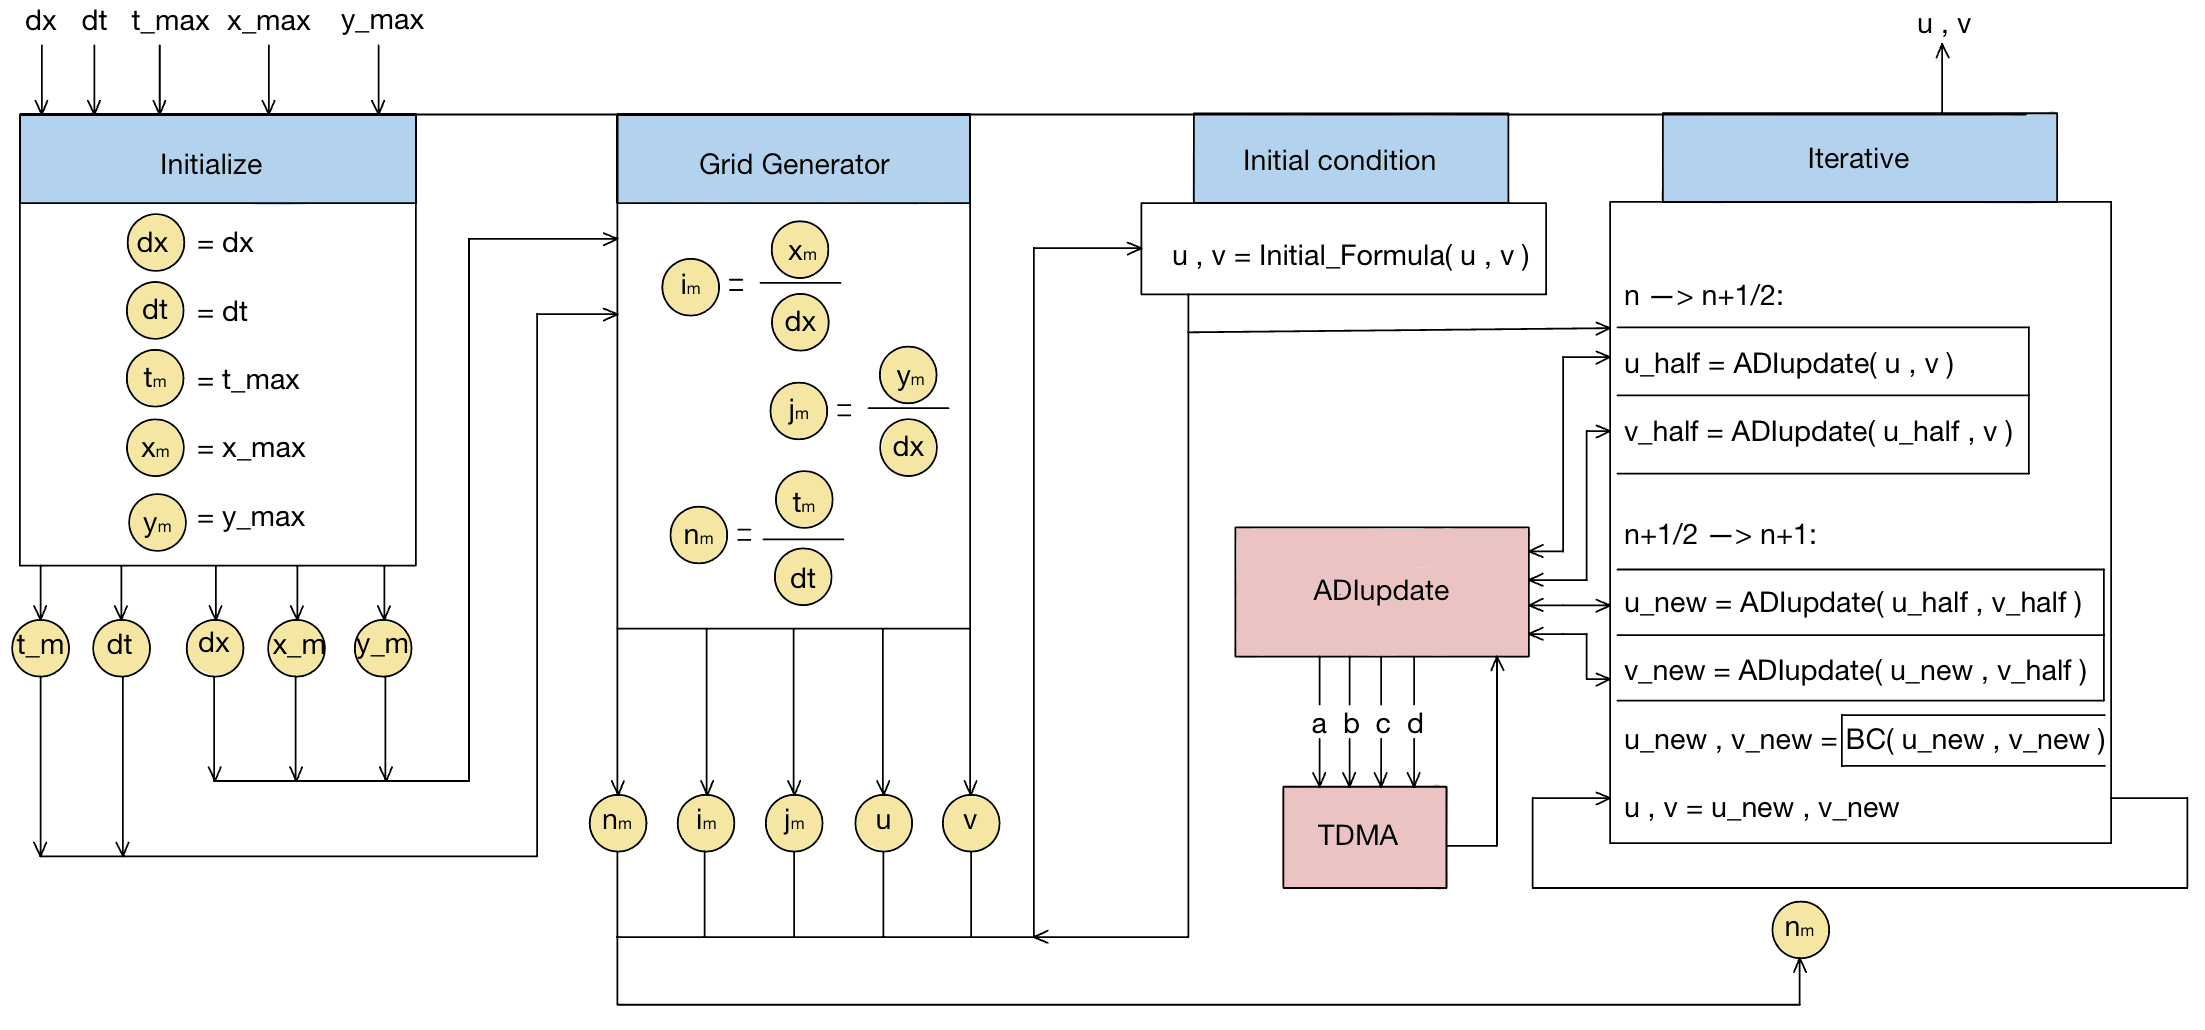
\includegraphics[width=1\textwidth]{figuresGeneral/Solver_Structure.jpg}
    \label{IGs.jpg}
    \caption{Solver Structure }
\end{figure}

Our solver structure is showing above, where the varible
in the circle (yellow) means private, and the private function
(blue) contains major solve steps.














\newpage

\section{3. Vorticity Contour Result}
\subsection{Result Shown}
Using $\Delta t = 0.001$, which let the scheme satisify stability condition,
we get the result for grid size= 0.02 is showing below:
\begin{figure}[H]
    \centering
    \begin{minipage}{\linewidth}
    \centering
    \begin{minipage}{0.5\textwidth}
    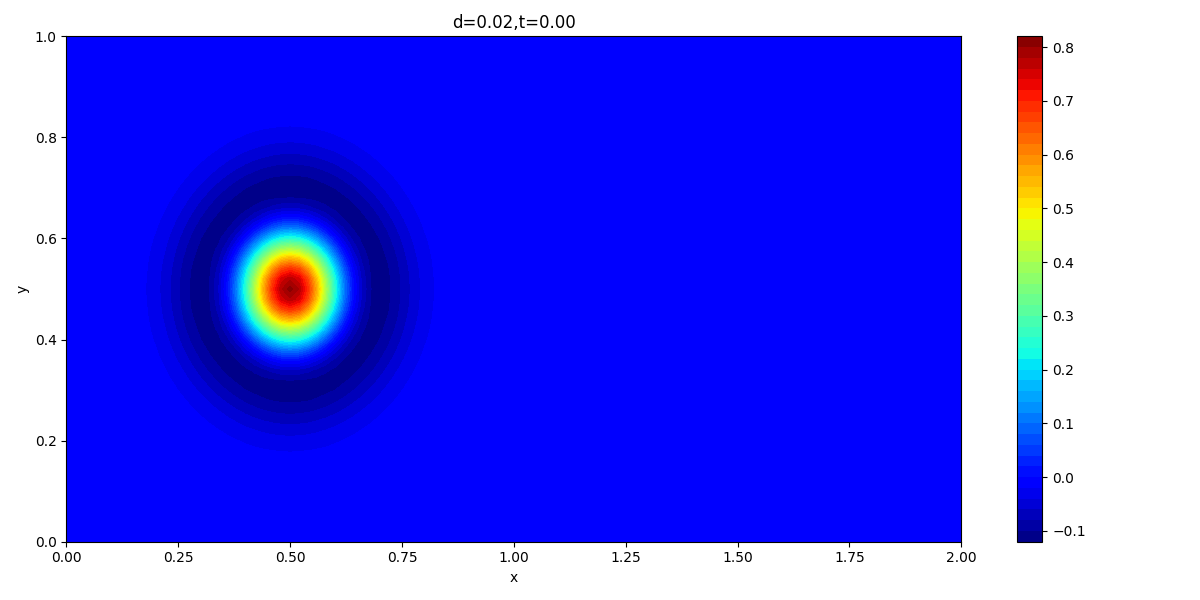
\includegraphics[width=\linewidth]{figures/3d0.02t0.00.png}
    \label{fig1}
    \end{minipage}\hfill
    \begin{minipage}{0.5\textwidth}
    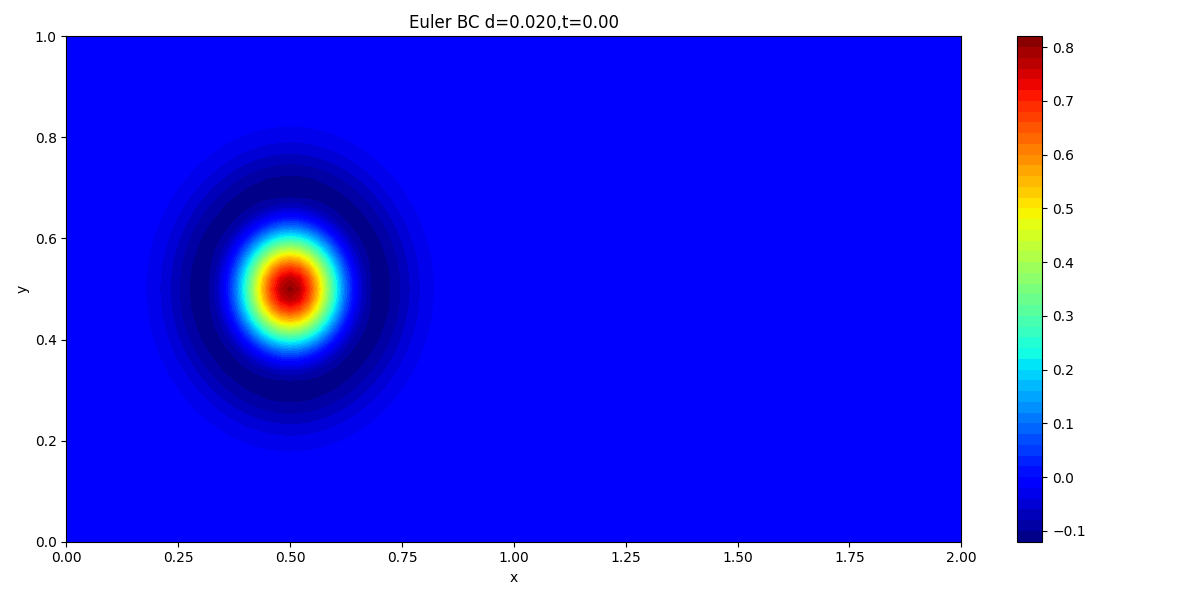
\includegraphics[width=\linewidth]{figures/3Ed0.020t0.00.png}
    \label{fig2}
    \end{minipage}
    \vspace{-1.5em}
    
    \begin{minipage}{0.5\textwidth}
    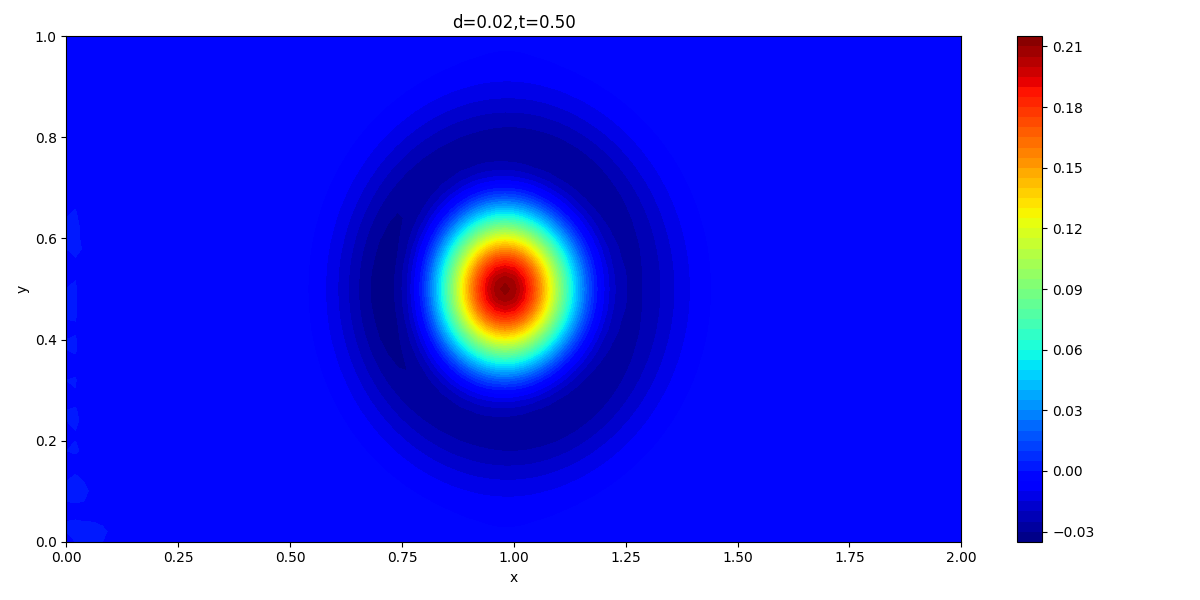
\includegraphics[width=\linewidth]{figures/3d0.02t0.50.png}
    \label{fig1}
    \end{minipage}\hfill
    \begin{minipage}{0.5\textwidth}
    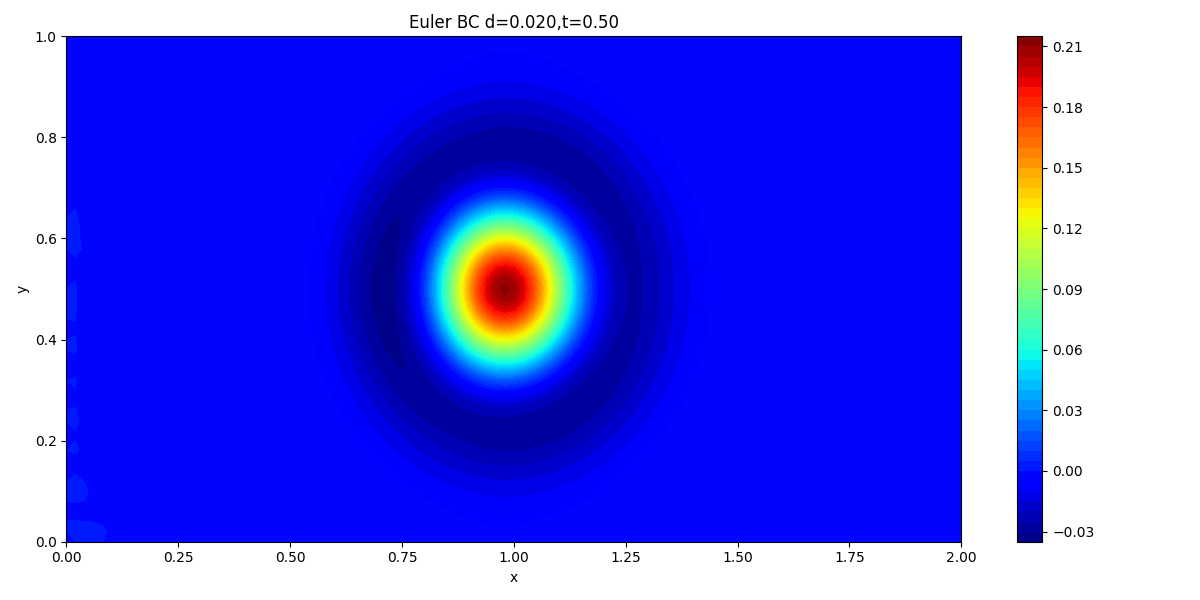
\includegraphics[width=\linewidth]{figures/3Ed0.020t0.50.png}
    \label{fig2}
    \end{minipage}
    \vspace{-1.5em}
    
    \begin{minipage}{0.5\textwidth}
    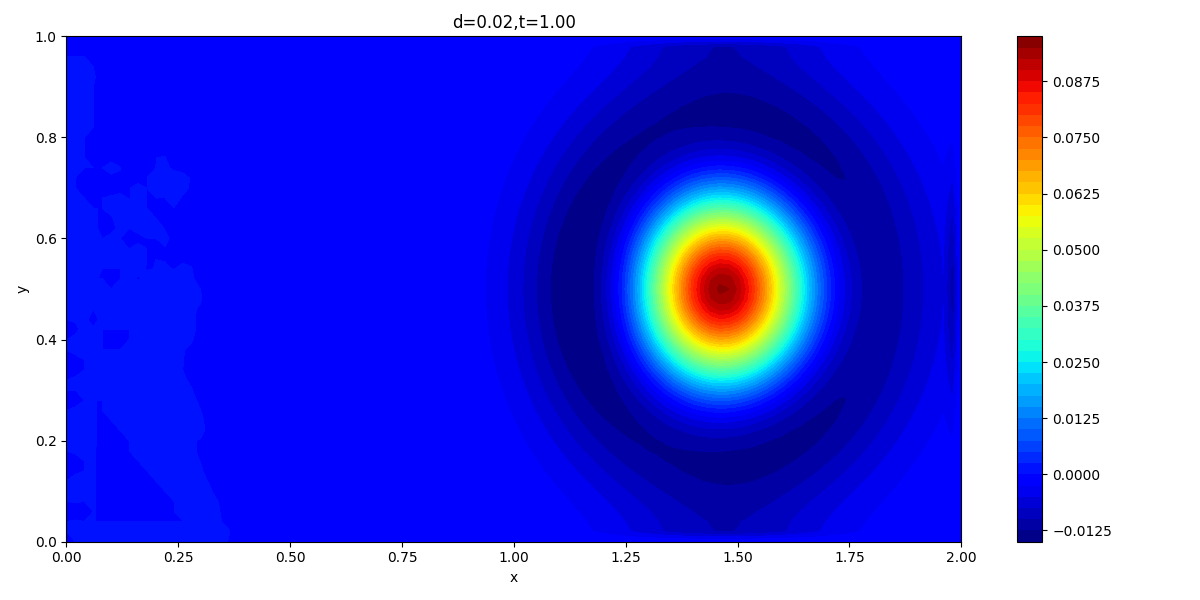
\includegraphics[width=\linewidth]{figures/3d0.02t1.00.png}
    \label{fig1}
    \end{minipage}\hfill
    \begin{minipage}{0.5\textwidth}
    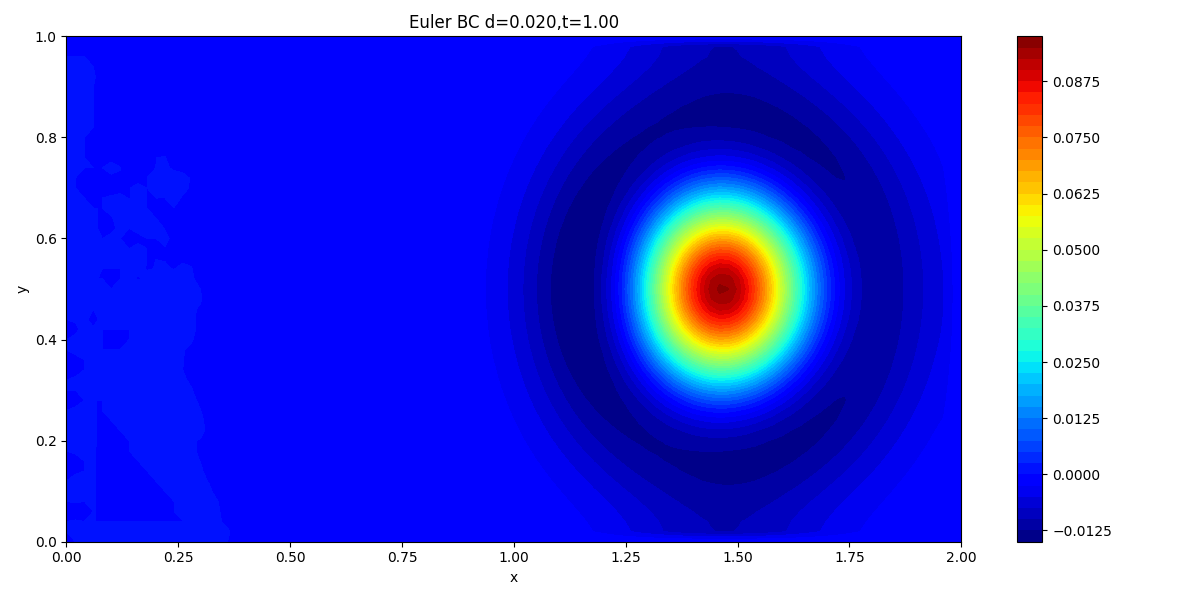
\includegraphics[width=\linewidth]{figures/3Ed0.020t1.00.png}
    \label{fig2}
    \end{minipage}
    \vspace{-1.5em}
    
    \begin{minipage}{0.5\textwidth}
    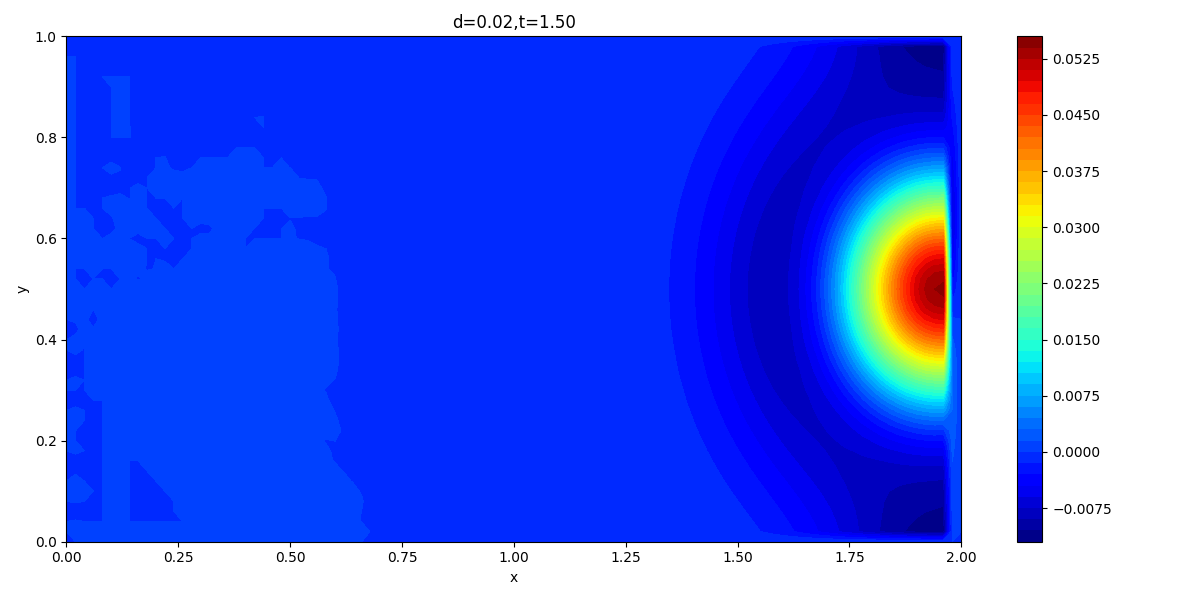
\includegraphics[width=\linewidth]{figures/3d0.02t1.50.png}
    \label{fig1}
    \end{minipage}\hfill
    \begin{minipage}{0.5\textwidth}
    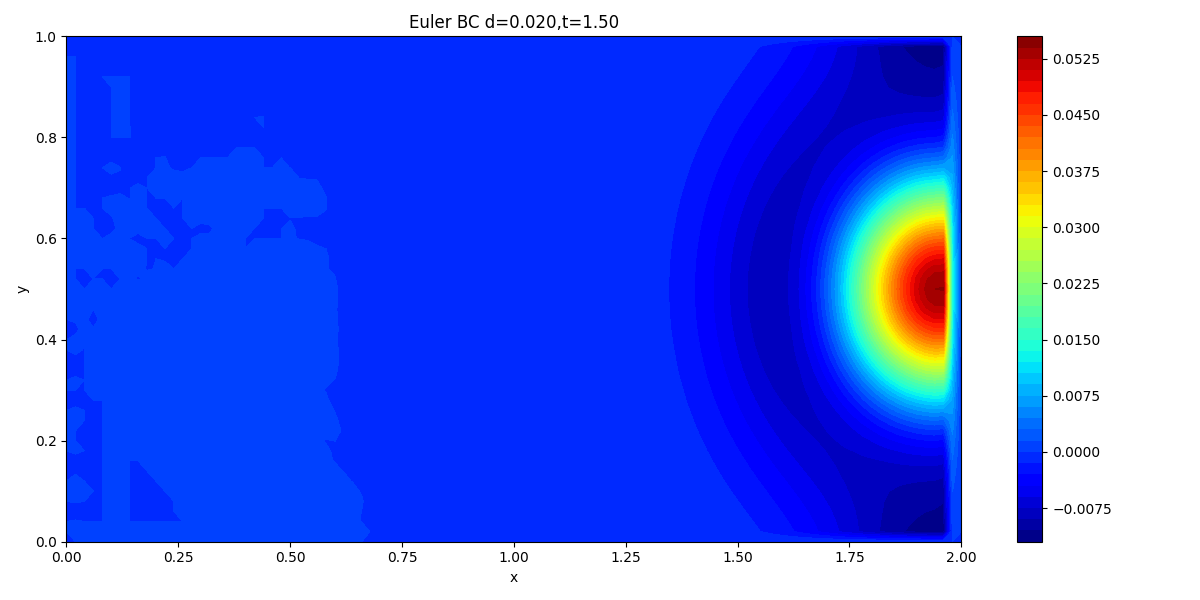
\includegraphics[width=\linewidth]{figures/3Ed0.020t1.50.png}
    \label{fig2}
    \end{minipage}
    \vspace{-1.5em}
    
    \begin{minipage}{0.5\textwidth}
    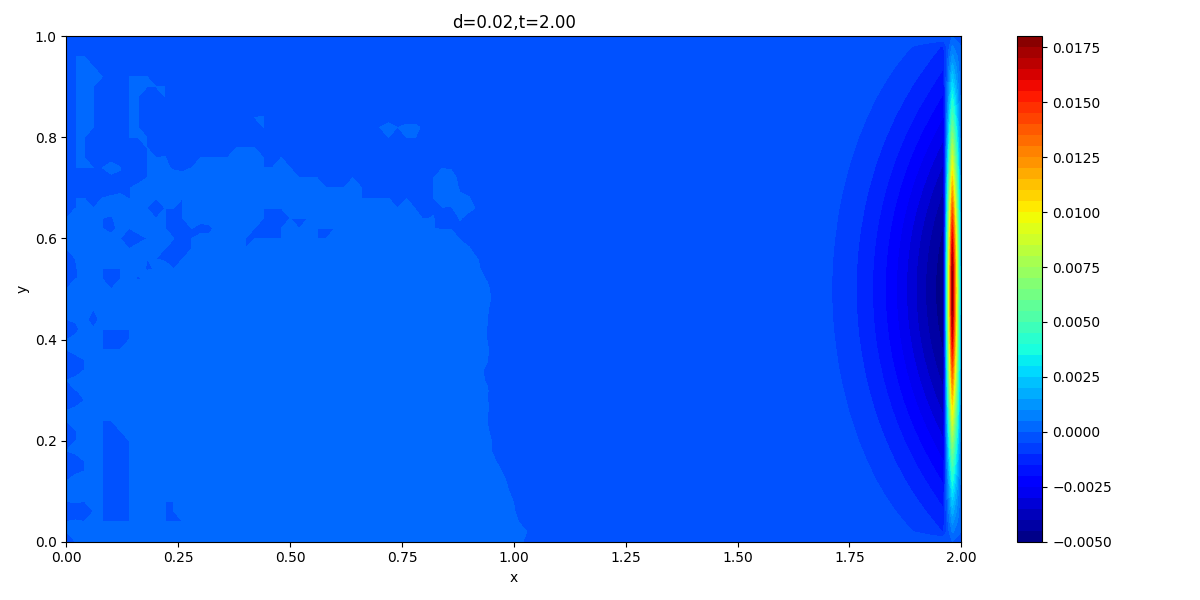
\includegraphics[width=\linewidth]{figures/3d0.02t2.00.png}
    \label{fig1}
    \end{minipage}\hfill
    \begin{minipage}{0.5\textwidth}
    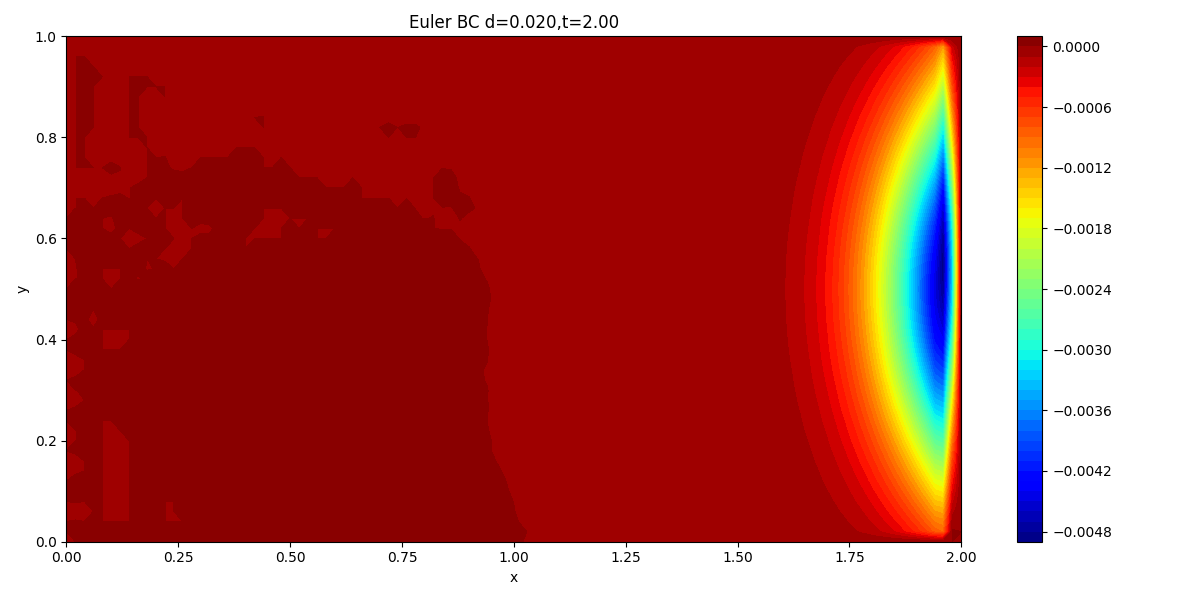
\includegraphics[width=\linewidth]{figures/3Ed0.020t2.00.png}
    \label{fig2}
    \end{minipage}
    \caption{Grid size 0.02, dirichlet BC vs Neumann BC}
    \end{minipage}
    
    \end{figure}

    Left is the 
    Dirichlet boundary condition(Boundary condition a), the 
    right side is Neumann boundary condition, time 0, 0.5, 1.0, 
    1.5, 2.0.
    
    For grid size 0.02, could see the vortex is moving from left
to right, and touch the right boundary at t=1.5. By compare 
the two boundary conditions, we could notice for Neumann 
boundary condition, the boundary effect on vortex is much
smaller than the result in Dirichlet boundary condition. The 
same observation on the finer grids:




\begin{figure}[H]
\centering
\begin{minipage}{\linewidth}
\centering
\begin{minipage}{0.5\textwidth}
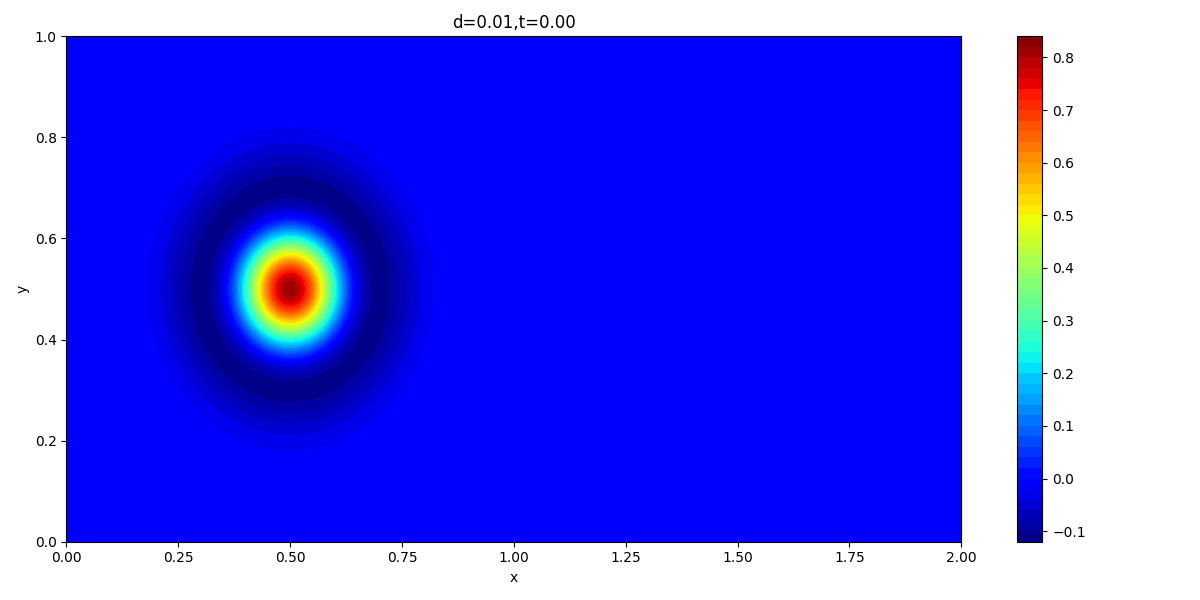
\includegraphics[width=\linewidth]{figures/3d0.01t0.00.png}
\label{fig1}
\end{minipage}\hfill
\begin{minipage}{0.5\textwidth}
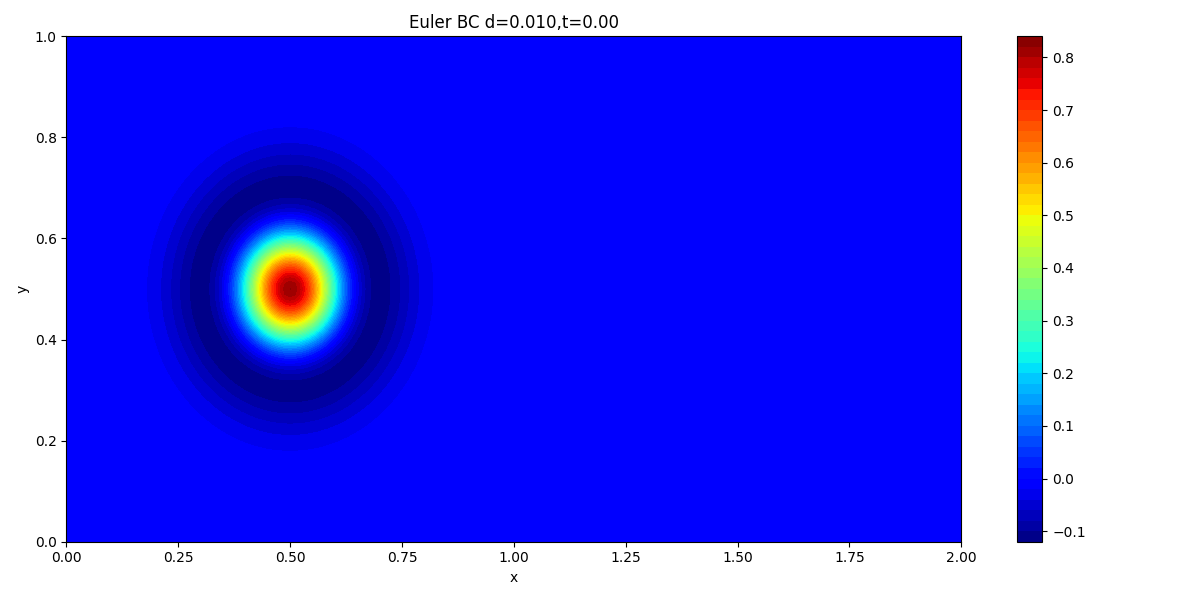
\includegraphics[width=\linewidth]{figures/3Ed0.010t0.00.png}
\label{fig2}
\end{minipage}
\vspace{-1.5em}

\begin{minipage}{0.5\textwidth}
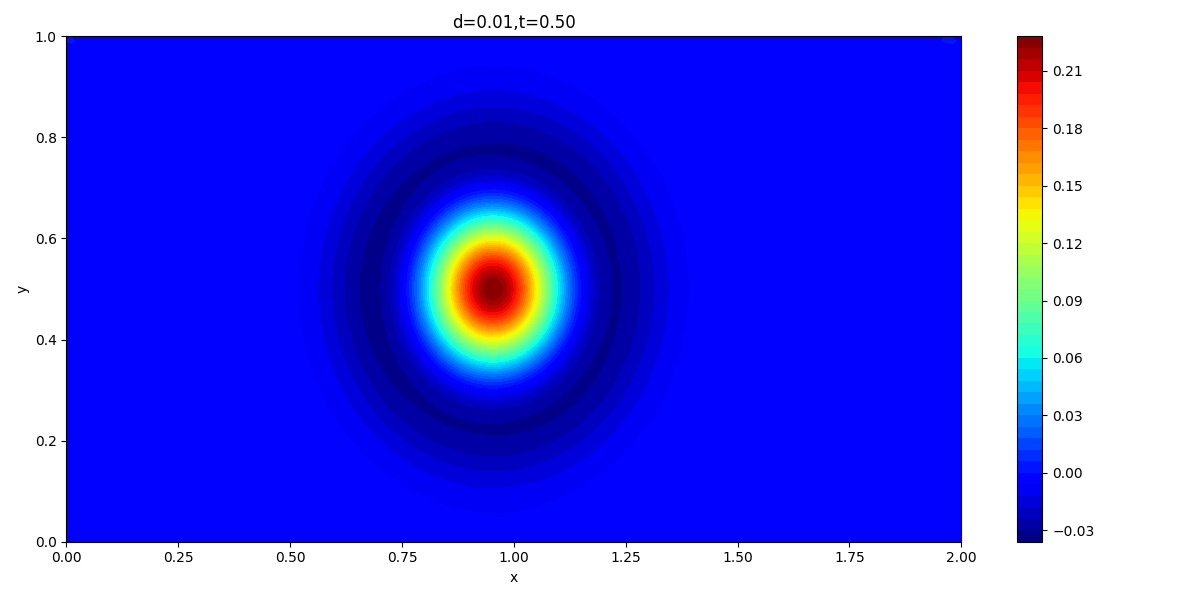
\includegraphics[width=\linewidth]{figures/3d0.01t0.50.png}
\label{fig3}
\end{minipage}\hfill
\begin{minipage}{0.5\textwidth}
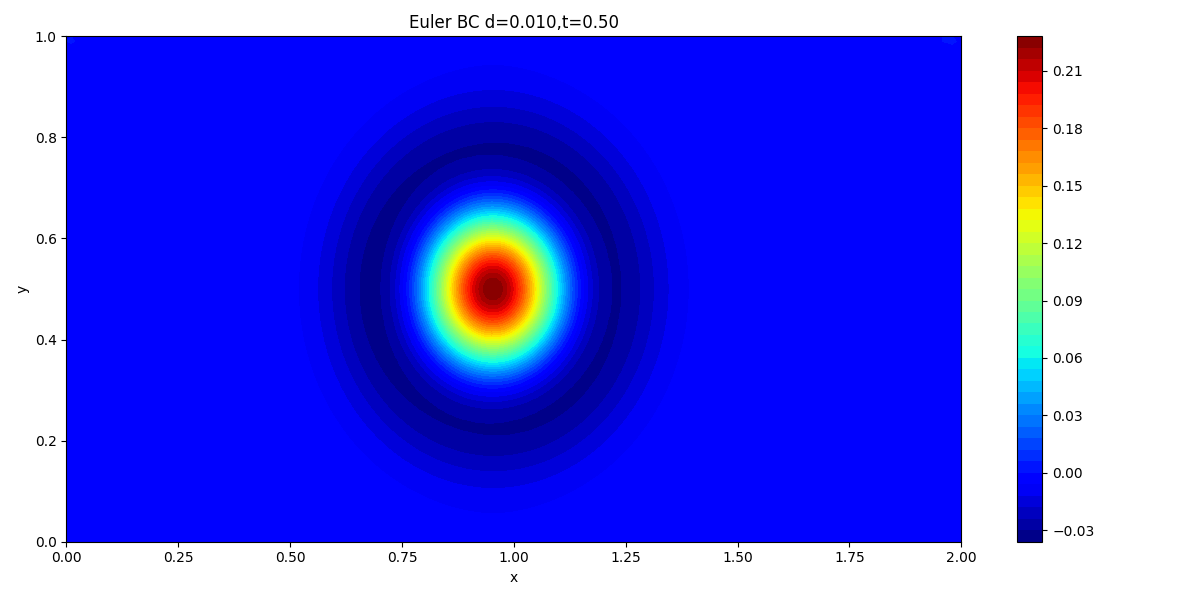
\includegraphics[width=\linewidth]{figures/3Ed0.010t0.50.png}
\label{fig4}
\end{minipage}
\vspace{-1.5em}

\begin{minipage}{0.5\textwidth}
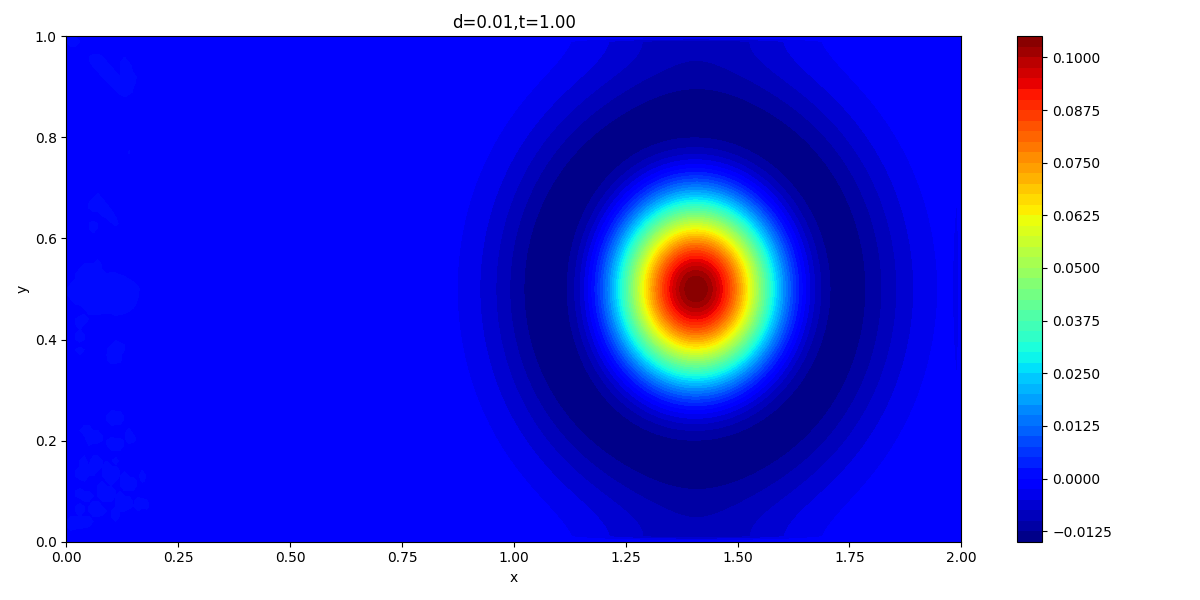
\includegraphics[width=\linewidth]{figures/3d0.01t1.00.png}
\label{fig5}
\end{minipage}\hfill
\begin{minipage}{0.5\textwidth}
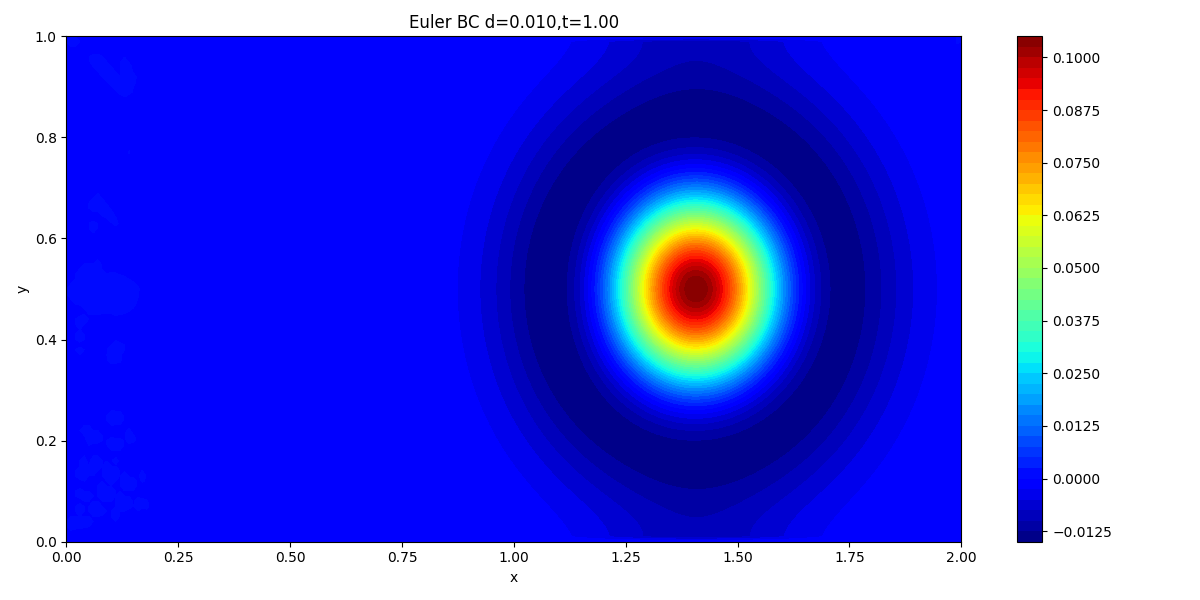
\includegraphics[width=\linewidth]{figures/3Ed0.010t1.00.png}
\label{fig6}
\end{minipage}
\vspace{-1.5em}

\begin{minipage}{0.5\textwidth}
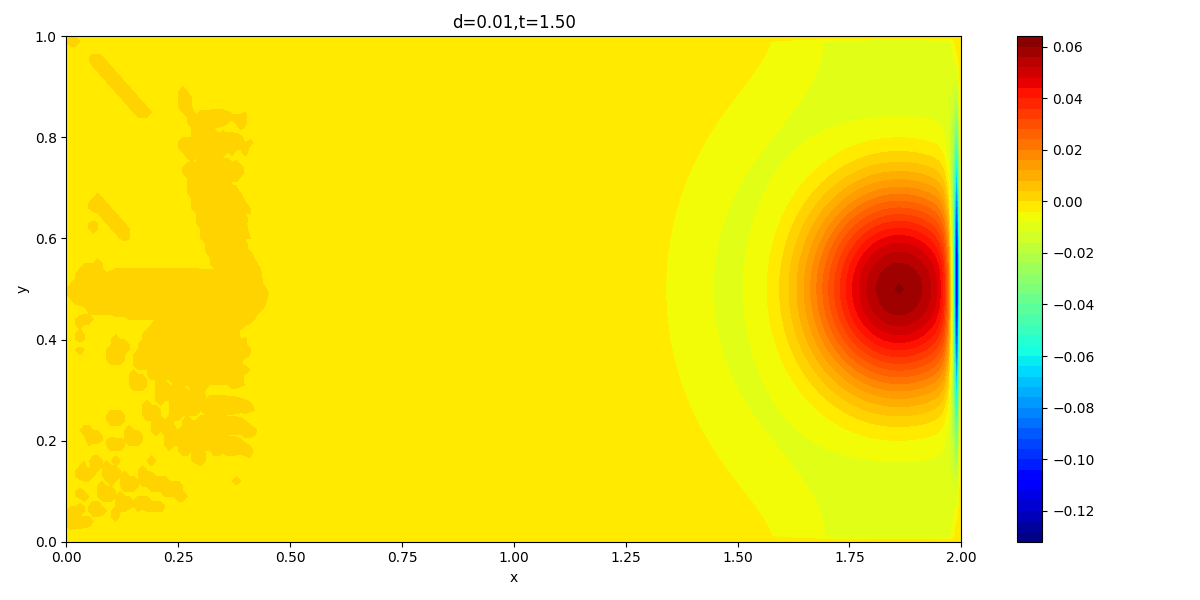
\includegraphics[width=\linewidth]{figures/3d0.01t1.50.png}
\label{fig7}
\end{minipage}\hfill
\begin{minipage}{0.5\textwidth}
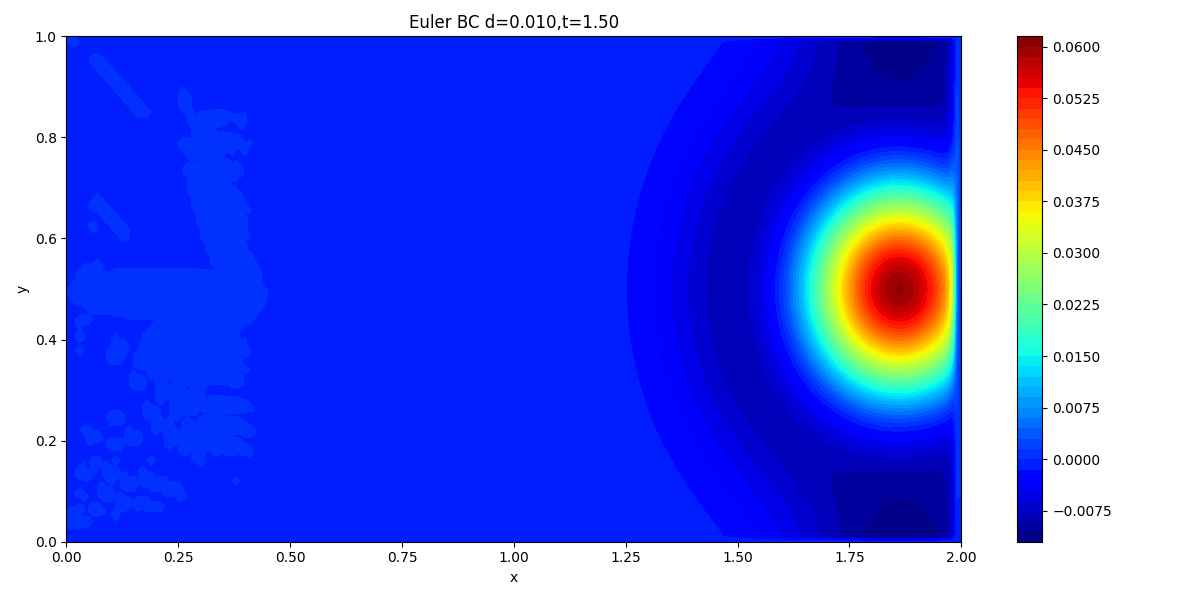
\includegraphics[width=\linewidth]{figures/3Ed0.010t1.50.png}
\label{fig8}
\end{minipage}
\vspace{-1.5em}

\begin{minipage}{0.5\textwidth}
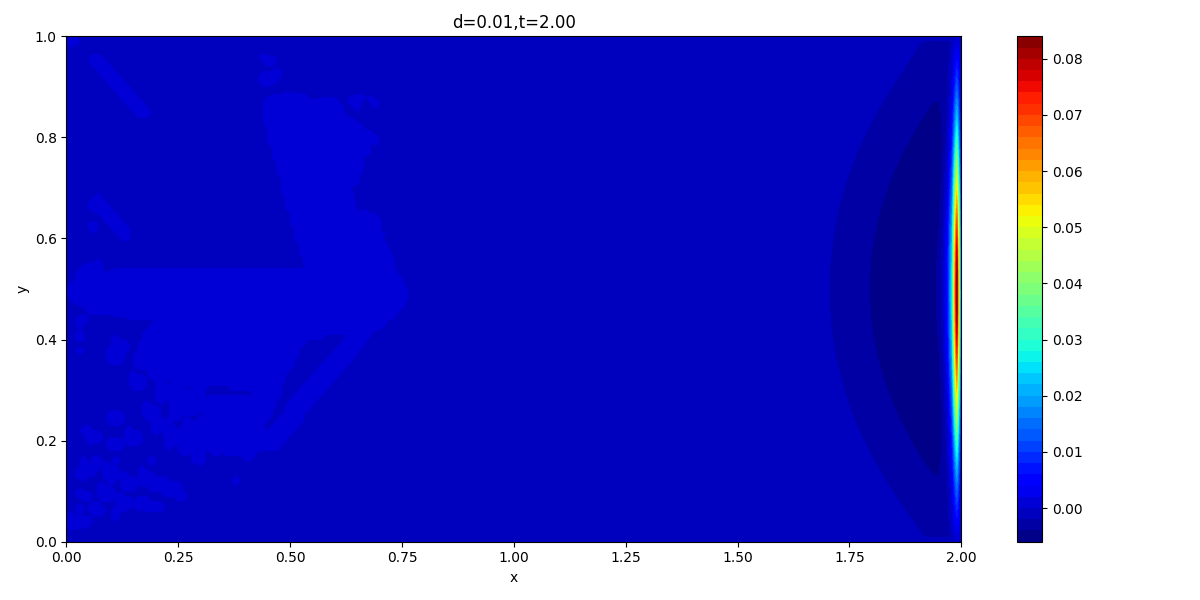
\includegraphics[width=\linewidth]{figures/3d0.01t2.00.png}
\label{fig9}
\end{minipage}\hfill
\begin{minipage}{0.5\textwidth}
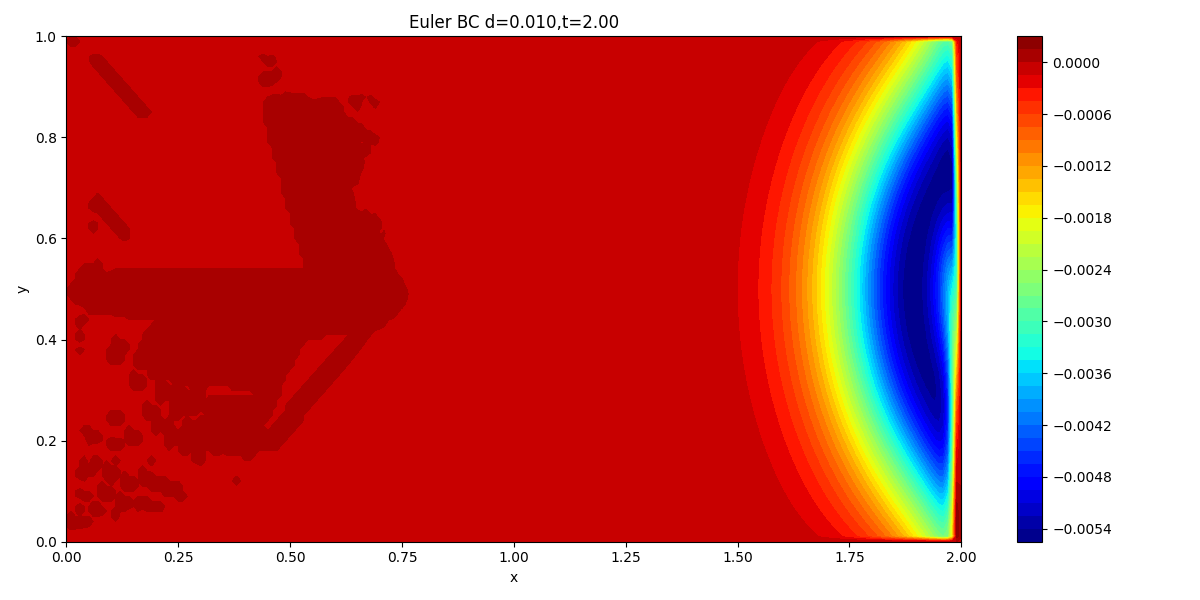
\includegraphics[width=\linewidth]{figures/3Ed0.010t2.00.png}
\label{fig10}
\end{minipage}
\caption{Grid size 0.01, dirichlet BC vs Neumann BC}

\end{minipage}
\end{figure}

For the finnest grid $\Delta = 0.005$, the result is much more 
accurate than the others, where we could see the vortex 
center's value(peak value) is larger than the other grids, and
the vortex influence region is smaller than other grids at the 
same time point.




\begin{figure}[H]
\centering
\begin{minipage}{\linewidth}
\centering
\begin{minipage}{0.5\textwidth}
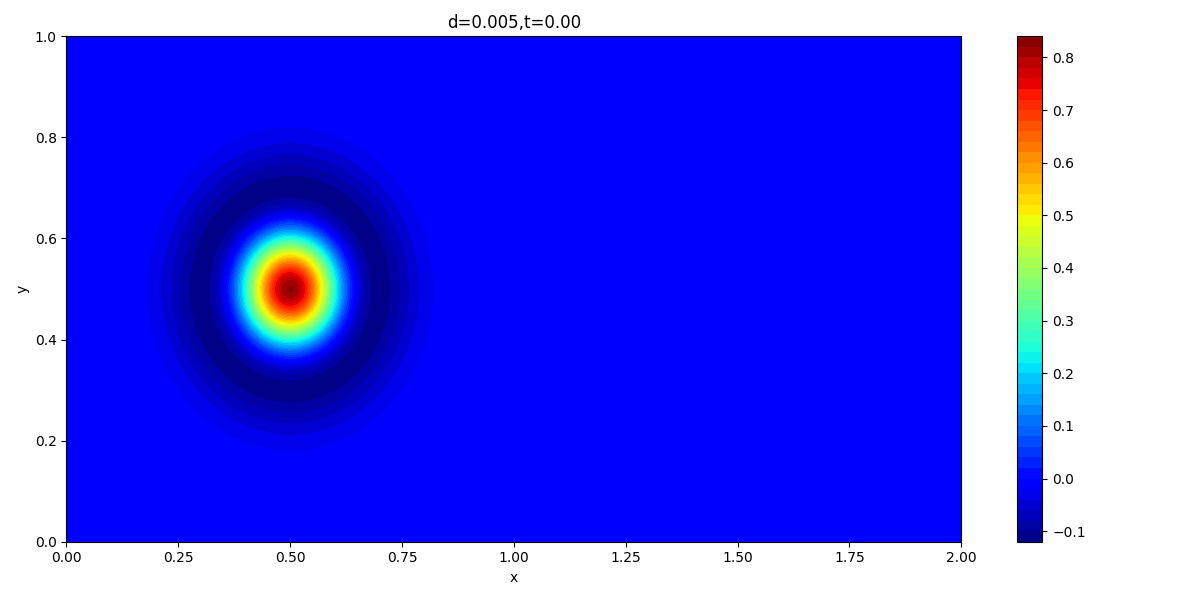
\includegraphics[width=\linewidth]{figures/3d0.005t0.00.png}
\label{fig1}
\end{minipage}\hfill
\begin{minipage}{0.5\textwidth}
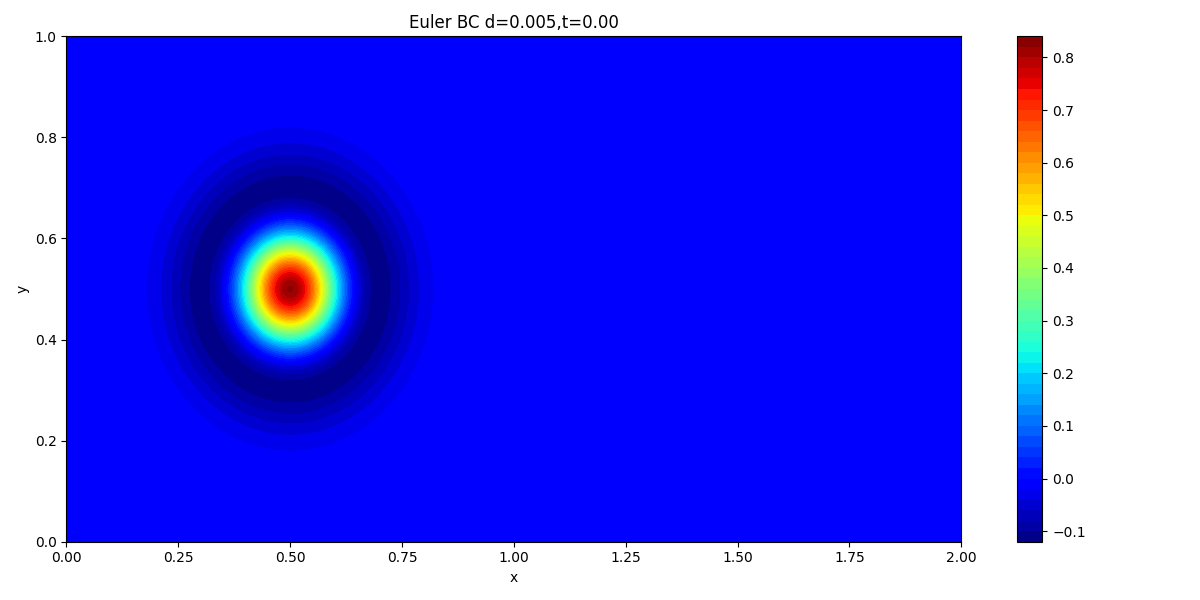
\includegraphics[width=\linewidth]{figures/3Ed0.005t0.00.png}
\label{fig2}
\end{minipage}
\vspace{-1.5em}

\begin{minipage}{0.5\textwidth}
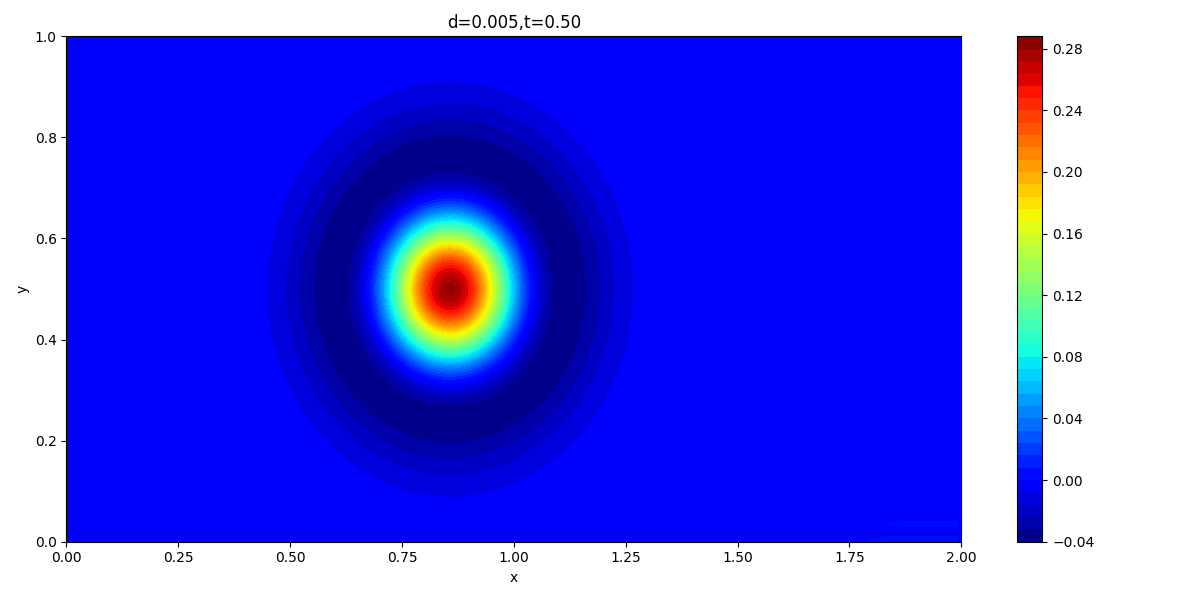
\includegraphics[width=\linewidth]{figures/3d0.005t0.50.png}
\label{fig3}
\end{minipage}\hfill
\begin{minipage}{0.5\textwidth}
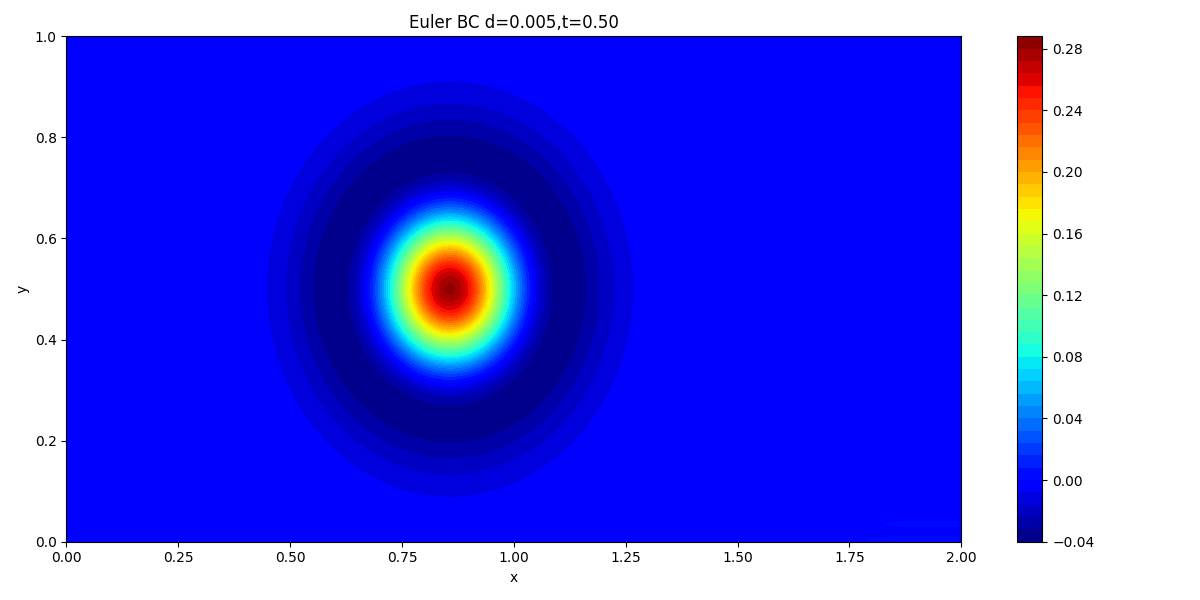
\includegraphics[width=\linewidth]{figures/3Ed0.005t0.50.png}
\label{fig4}
\end{minipage}
\vspace{-1.5em}

\begin{minipage}{0.5\textwidth}
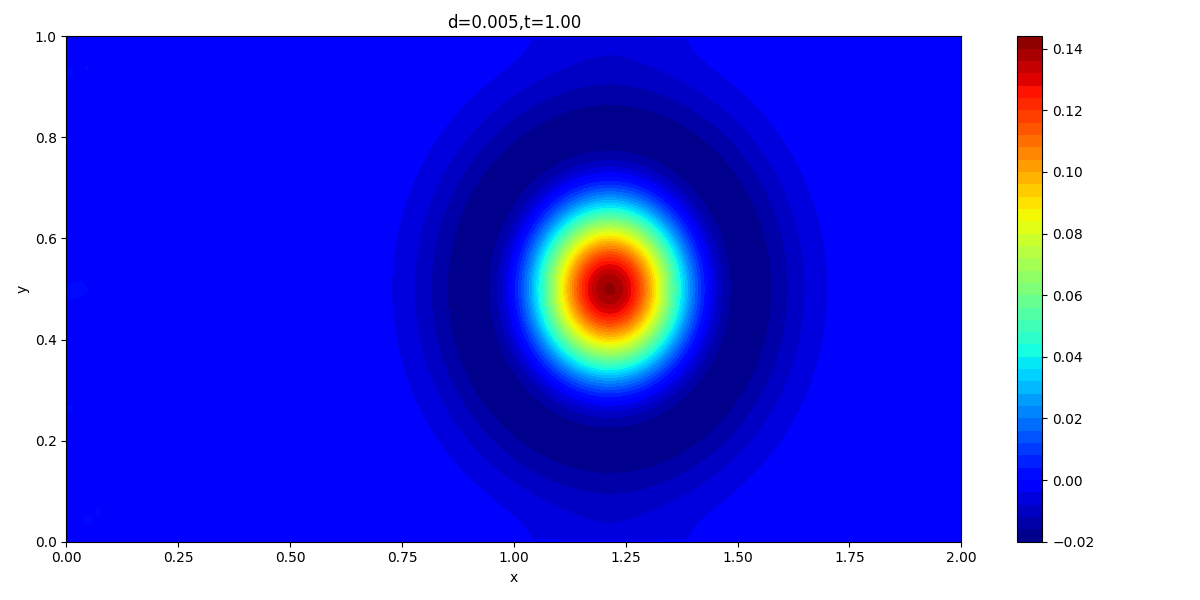
\includegraphics[width=\linewidth]{figures/3d0.005t1.00.png}
\label{fig5}
\end{minipage}\hfill
\begin{minipage}{0.5\textwidth}
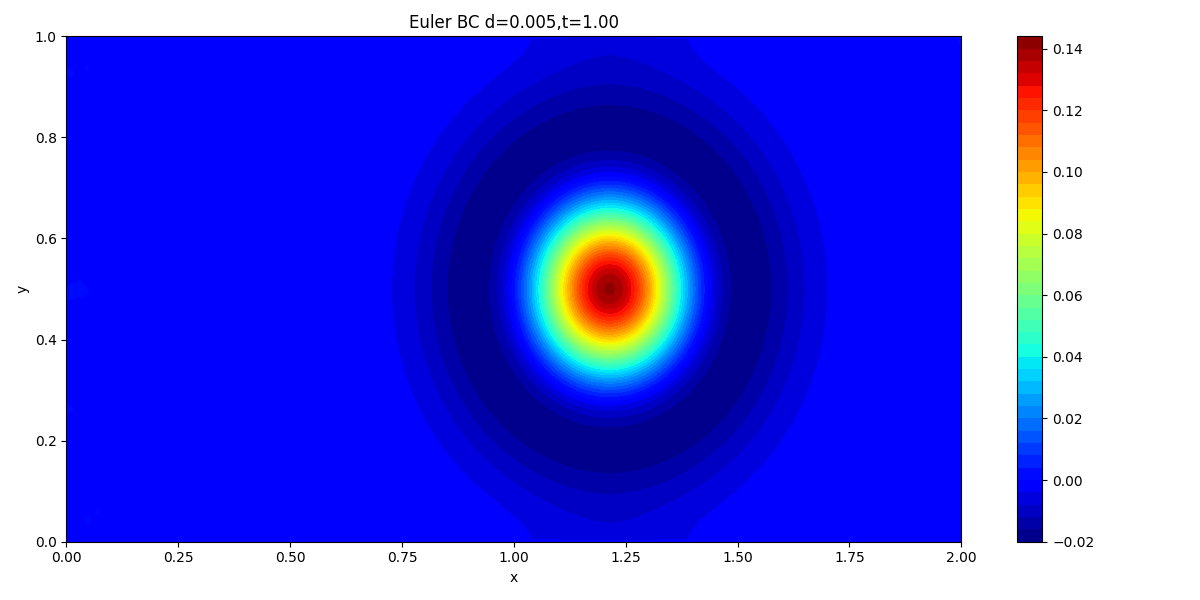
\includegraphics[width=\linewidth]{figures/3Ed0.005t1.00.png}
\label{fig6}
\end{minipage}
\vspace{-1.5em}

\begin{minipage}{0.5\textwidth}
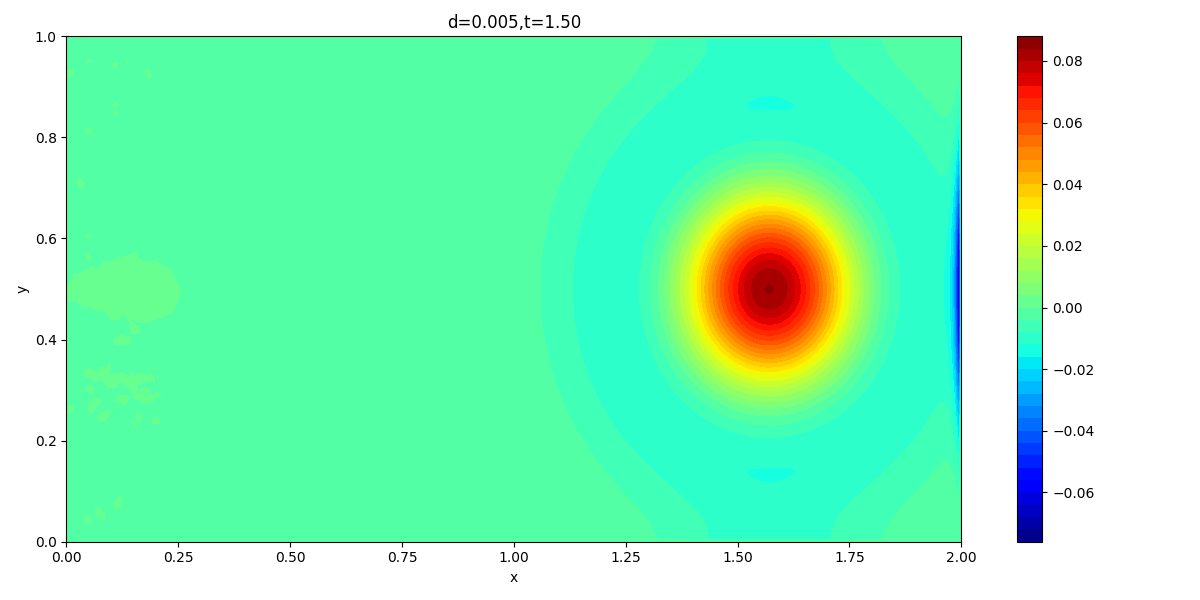
\includegraphics[width=\linewidth]{figures/3d0.005t1.50.png}
\label{fig7}
\end{minipage}\hfill
\begin{minipage}{0.5\textwidth}
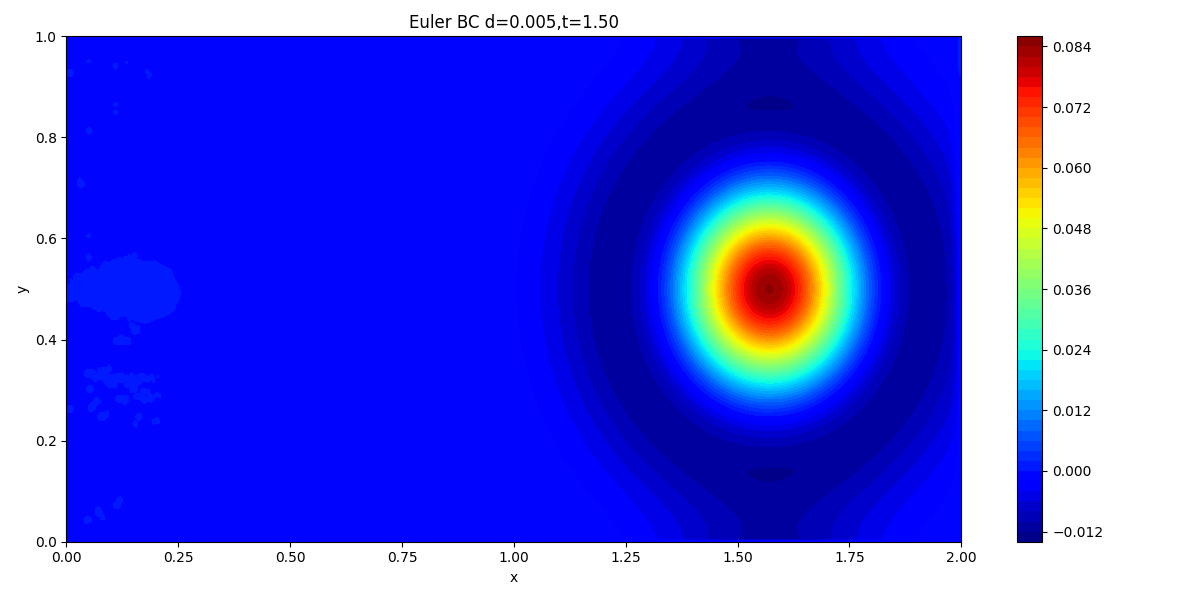
\includegraphics[width=\linewidth]{figures/3Ed0.005t1.50.png}
\label{fig8}
\end{minipage}
\vspace{-1.5em}

\begin{minipage}{0.5\textwidth}
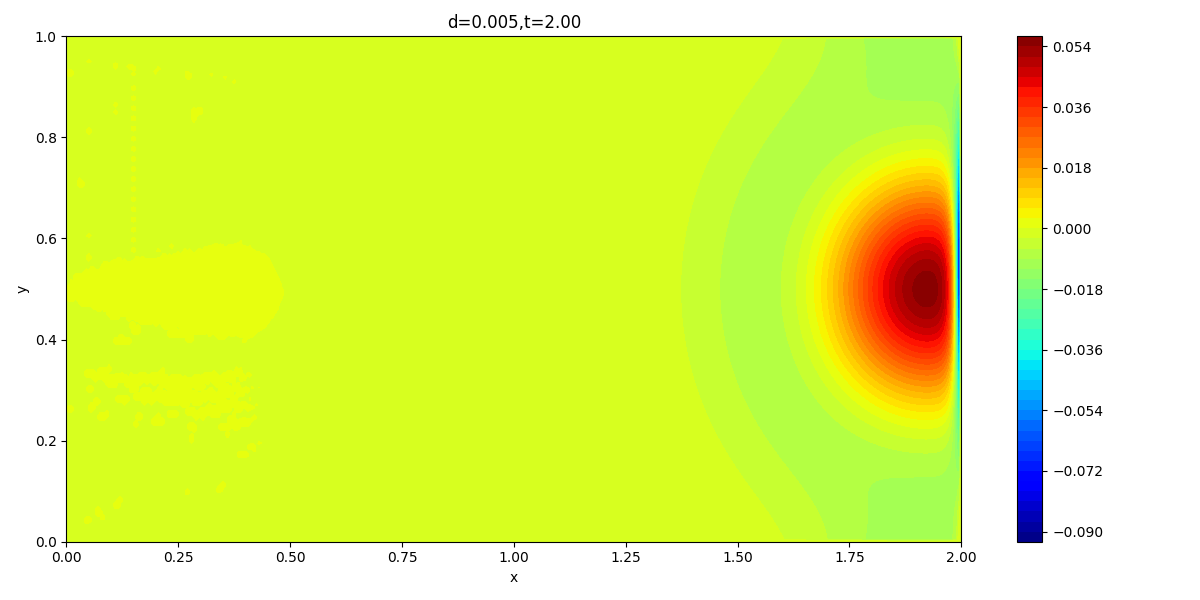
\includegraphics[width=\linewidth]{figures/3d0.005t2.00.png}
\label{fig9}
\end{minipage}\hfill
\begin{minipage}{0.5\textwidth}
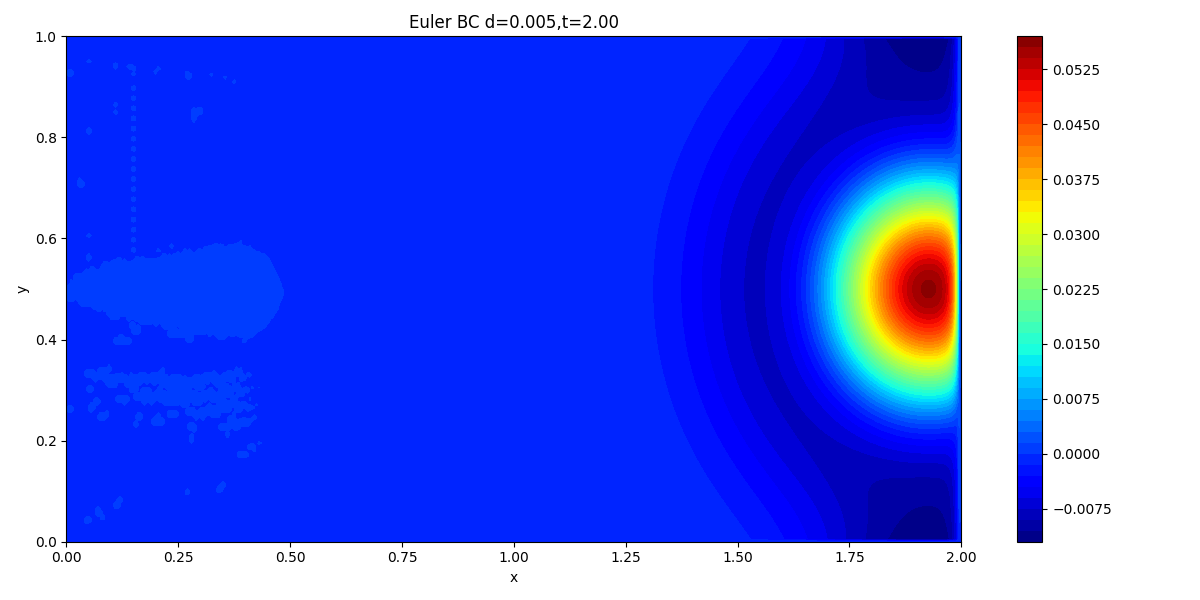
\includegraphics[width=\linewidth]{figures/3Ed0.005t2.00.png}
\label{fig10}
\end{minipage}
\caption{Grid size 0.005, dirichlet BC vs Neumann BC}

\end{minipage}
\end{figure}


\subsection{Observation}

\subsubsection{Comparsion among time}
Based on the result among different time, we could observe
the vortex moving from left to right, while 
the vortex effective range is getting biggere and bigger, 
and the amplitiude of the vortez center is decreasing. 

\begin{figure}[H]
    \centering
    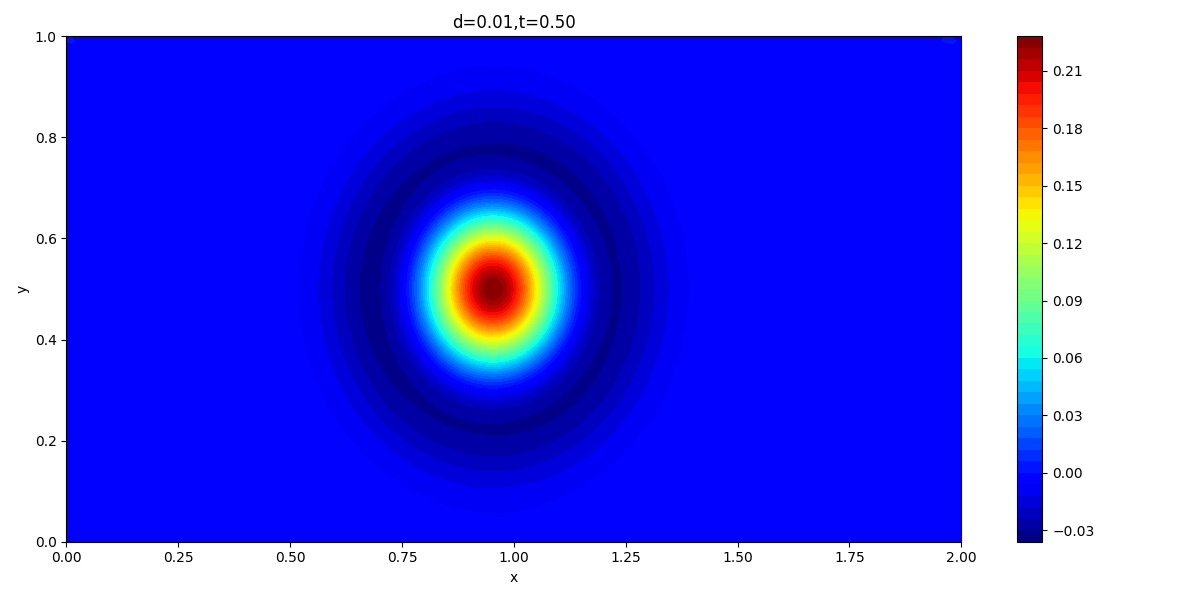
\includegraphics[width=0.48\linewidth]{figures/3d0.01t0.50.png}
    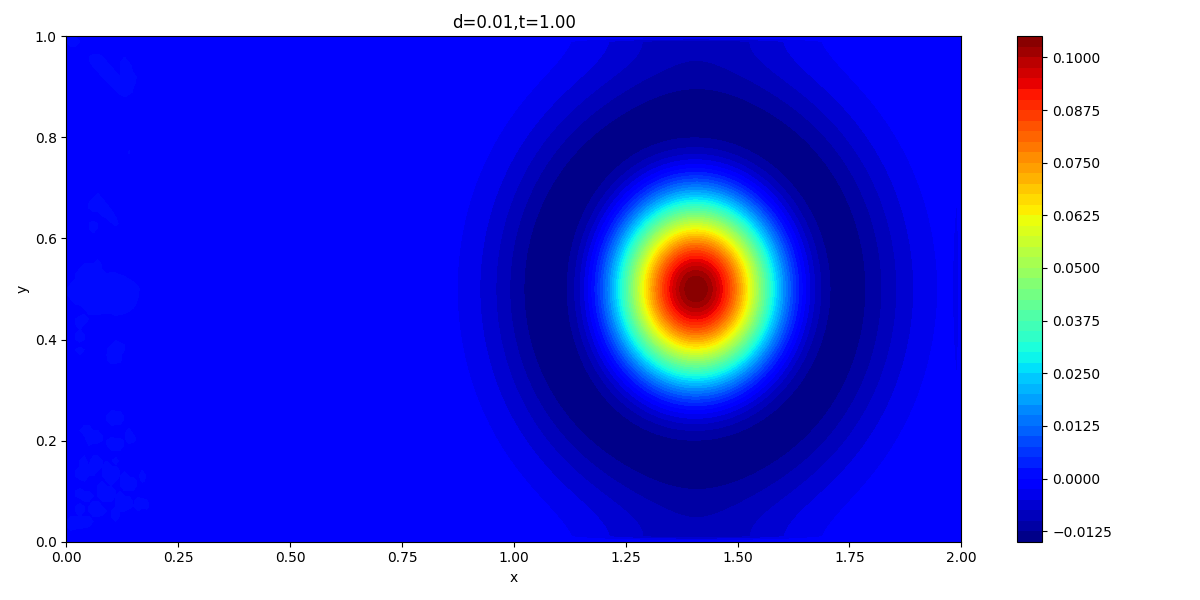
\includegraphics[width=0.48\linewidth]{figures/3d0.01t1.00.png}
    \label{IGs.jpg}
    \caption{Comparsion of t=0.5 and t=0.1, grid d=0.01}
\end{figure}




\subsubsection{Comparsion of different BC}

We have examined two different boundary condition (BC), one 
is Dirichlet boundary condition, where its right boundary its 
been artifically set to $u=1, v=0$, and Neumann boundary condition,
where at the boundary, the $u$ and $v$ gradience normal to the 
boundary is zero.\\

By compare the left (Dirichlet BC) and right (Neumann BC), 
we could see the boundary effection on the vortex at Neumann
BC is smaller than Dirichlet BC.


\begin{figure}[H]
    \centering
    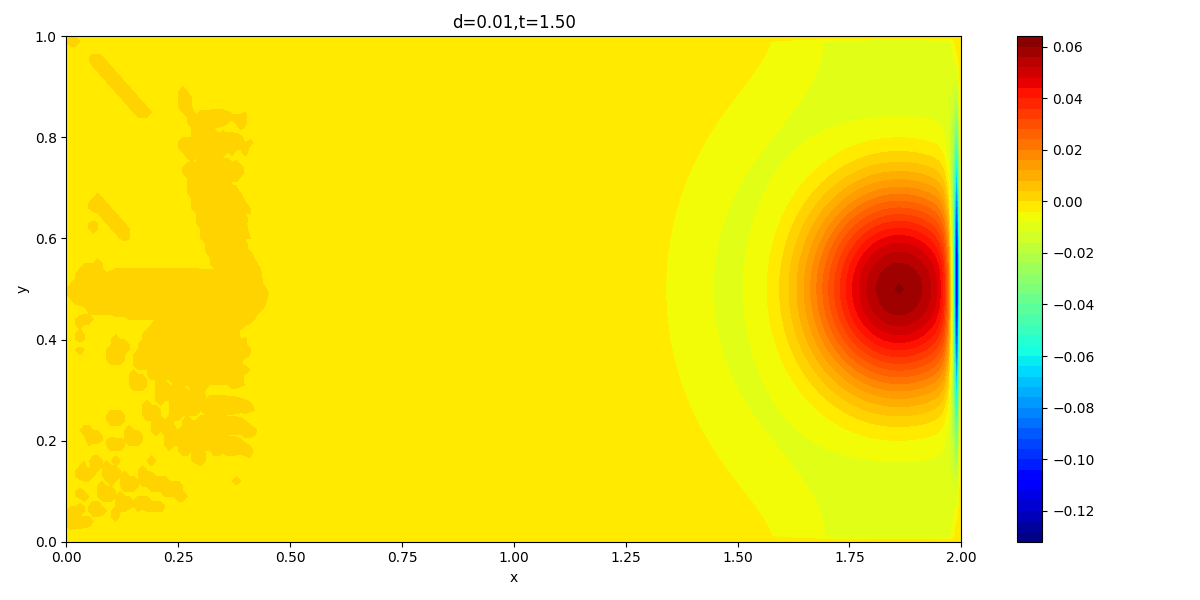
\includegraphics[width=0.48\linewidth]{figures/3d0.01t1.50.png}
    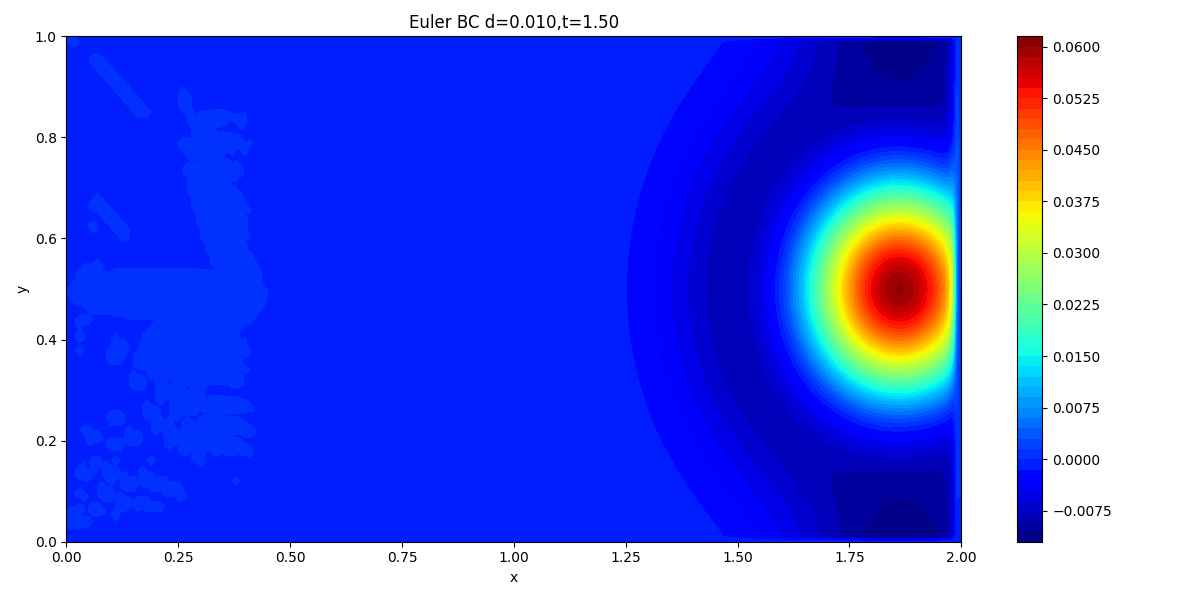
\includegraphics[width=0.48\linewidth]{figures/3Ed0.010t1.50.png}
    \label{IGs.jpg}
    \caption{Comparsion of Dirichlet BC and Neumann BC at t=1.5}
\end{figure}





\subsubsection{Comparsion of different grid size}
As showing above, we have examined the grid size at 0.02, 0.01
, and 0.005. Compare different grid size's result, could find the finer grid
as, the slower the diffusion speed it get.
%%%%%%%%%%%% MIGHT BE PROBLEM!!!!






\newpage
\section{4.  Vorticity Contour Result at $\mu = 0.001$}

\subsection{Result shown}
Changing $\mu$ from 0.01 to 0.001, the result in different size
grid is showing below:



\begin{figure}[H]
    \centering
    \begin{minipage}{\linewidth}
    \centering
    \begin{minipage}{0.5\textwidth}
    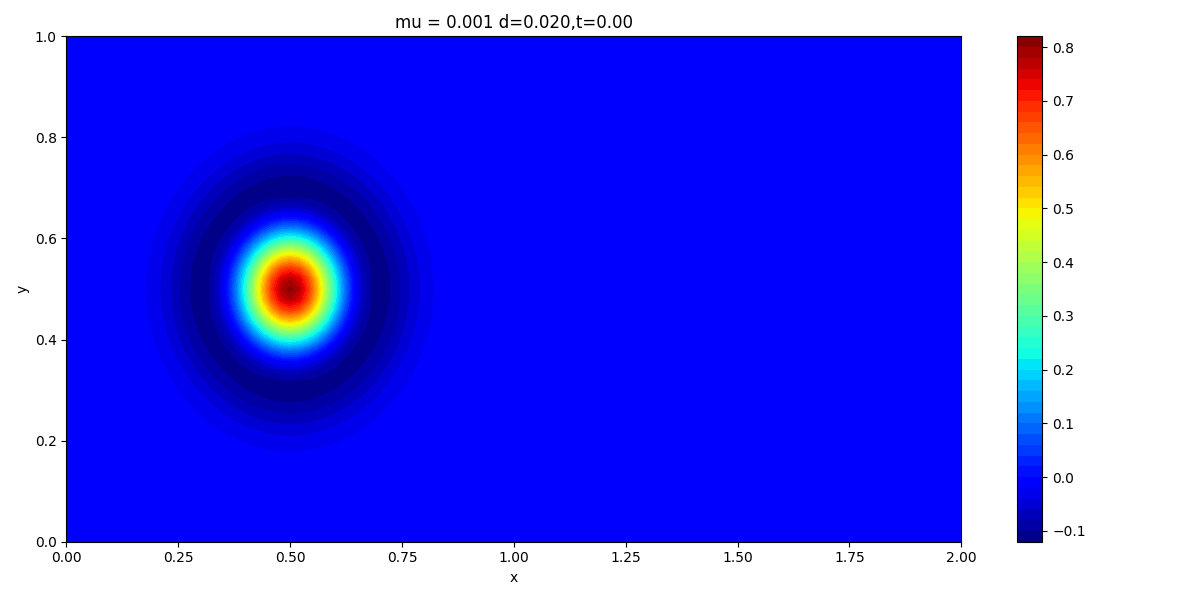
\includegraphics[width=\linewidth]{figuresmu/mu3d0.020t0.00.png}
    \label{fig1}
    \end{minipage}\hfill
    \begin{minipage}{0.5\textwidth}
    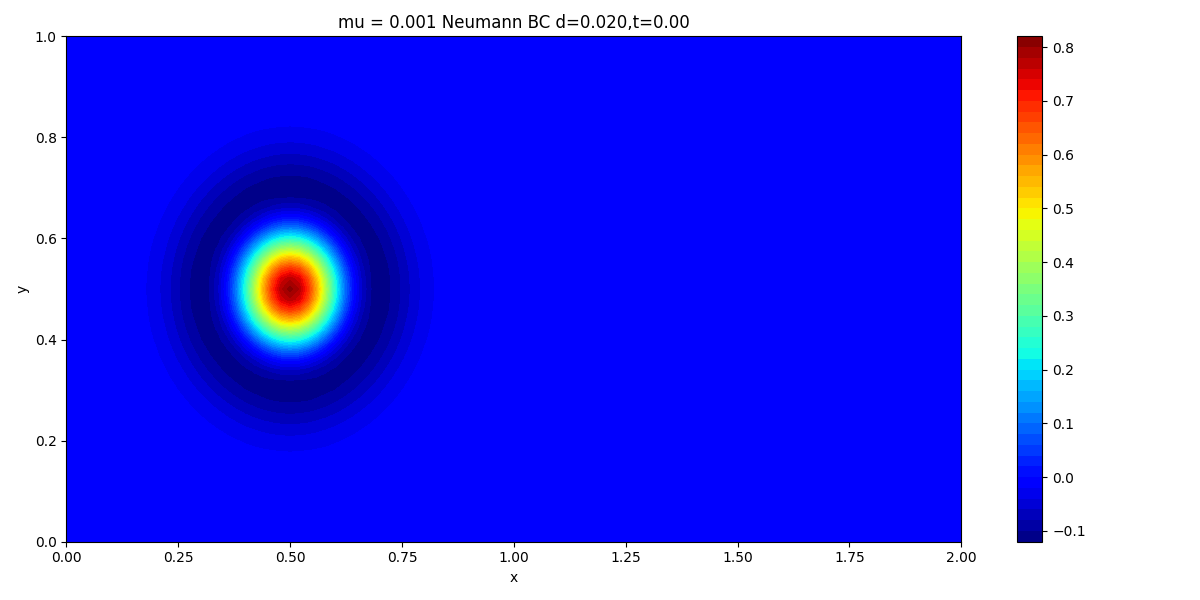
\includegraphics[width=\linewidth]{figuresmu/mu3Nud0.020t0.00.png}
    \label{fig2}
    \end{minipage}
    \vspace{-1.5em}
    
    \begin{minipage}{0.5\textwidth}
    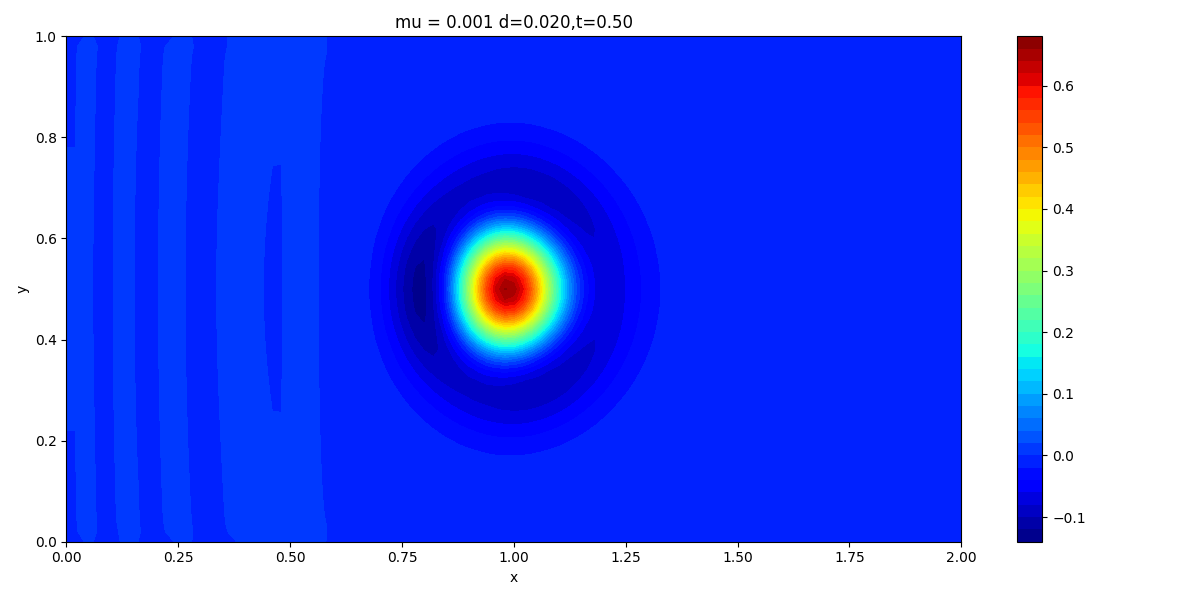
\includegraphics[width=\linewidth]{figuresmu/mu3d0.020t0.50.png}
    \label{fig3}
    \end{minipage}\hfill
    \begin{minipage}{0.5\textwidth}
    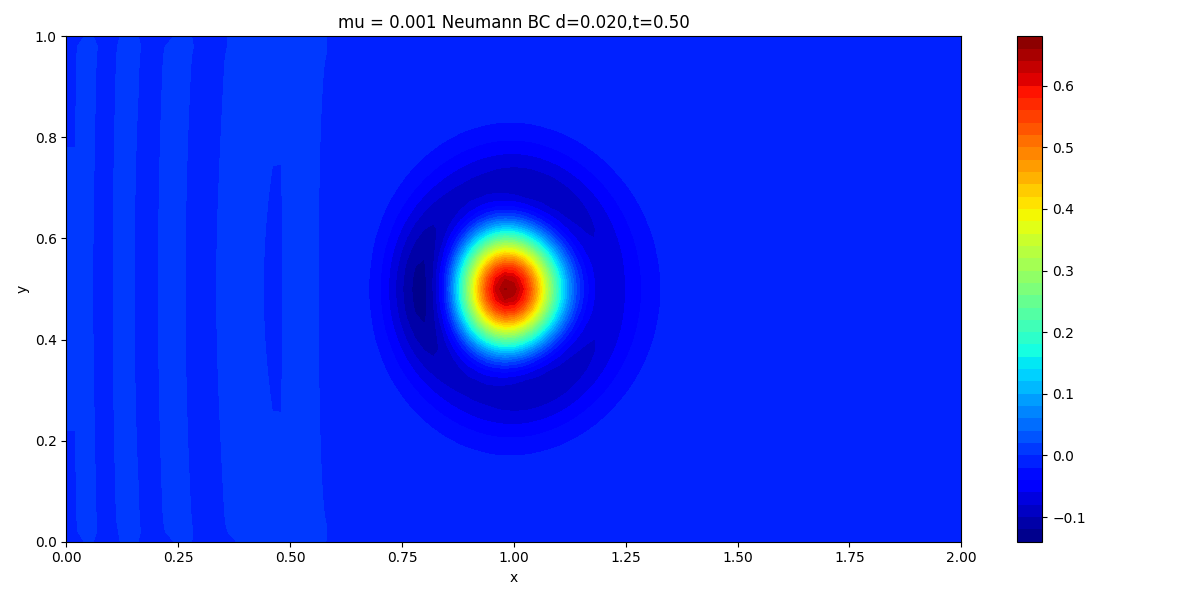
\includegraphics[width=\linewidth]{figuresmu/mu3Nud0.020t0.50.png}
    \label{fig4}
    \end{minipage}
    \vspace{-1.5em}
    
    \begin{minipage}{0.5\textwidth}
    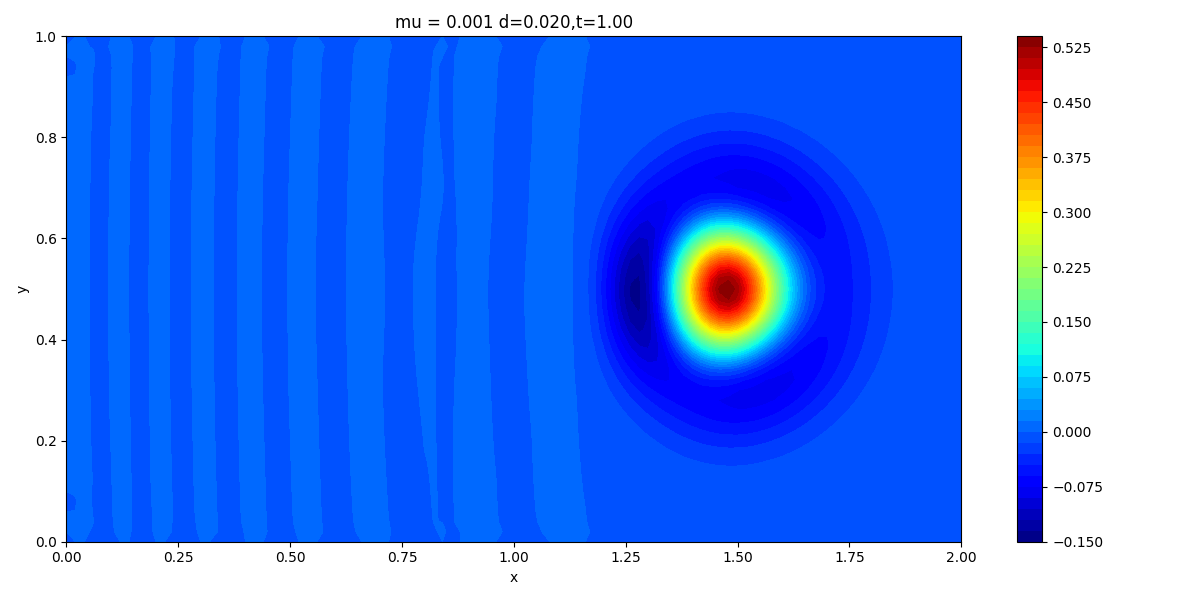
\includegraphics[width=\linewidth]{figuresmu/mu3d0.020t1.00.png}
    \label{fig5}
    \end{minipage}\hfill
    \begin{minipage}{0.5\textwidth}
    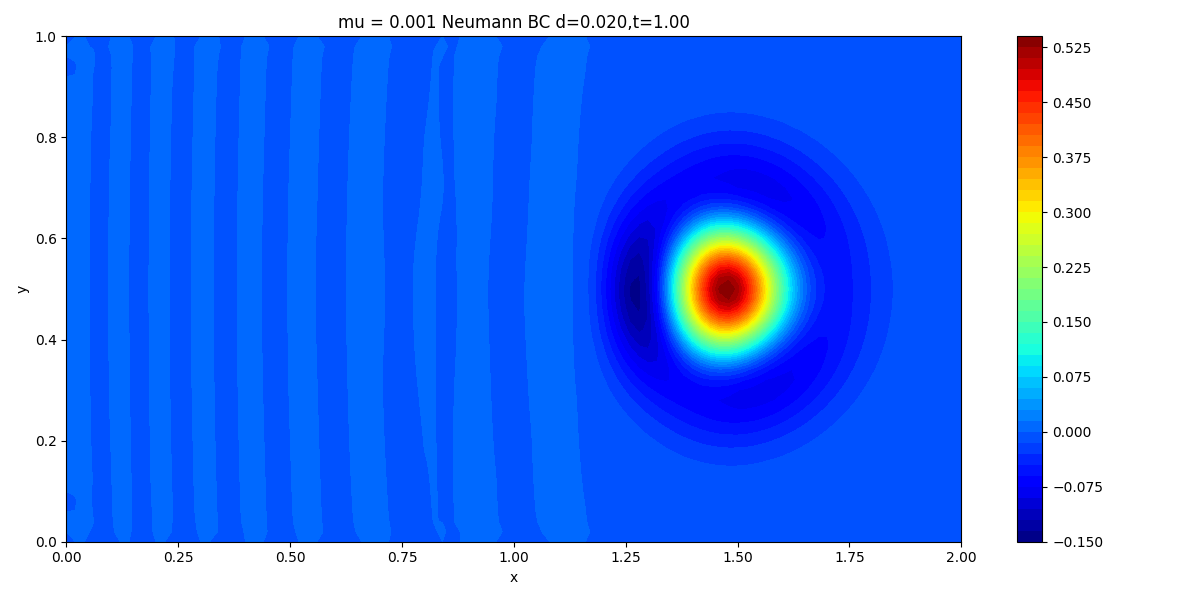
\includegraphics[width=\linewidth]{figuresmu/mu3Nud0.020t1.00.png}
    \label{fig6}
    \end{minipage}
    \vspace{-1.5em}
    
    \begin{minipage}{0.5\textwidth}
    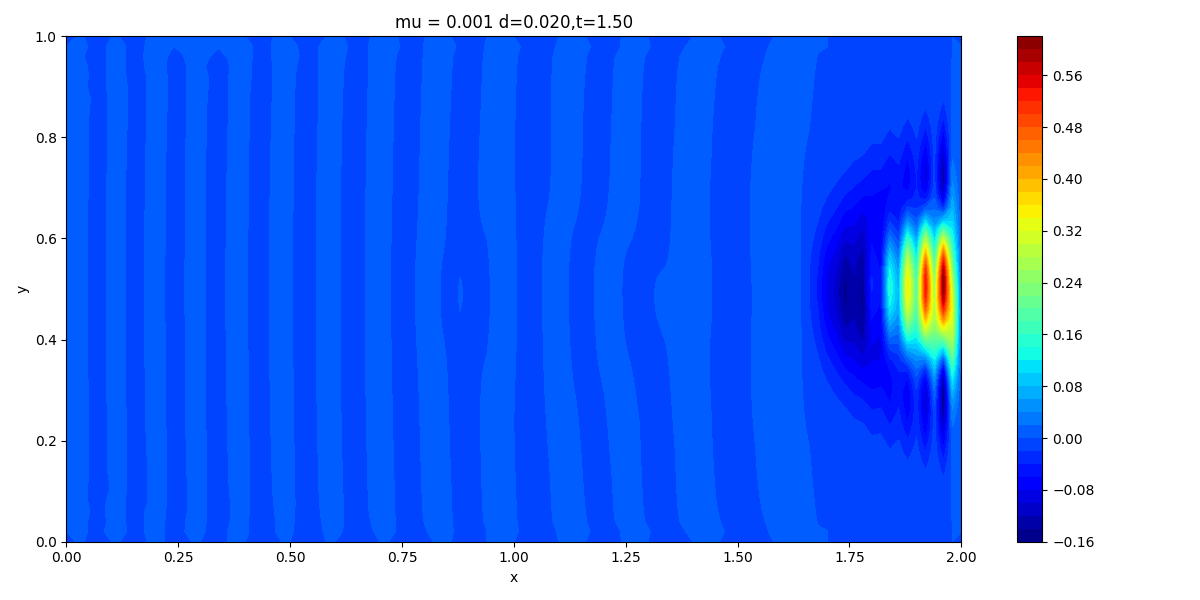
\includegraphics[width=\linewidth]{figuresmu/mu3d0.020t1.50.png}
    \label{fig7}
    \end{minipage}\hfill
    \begin{minipage}{0.5\textwidth}
    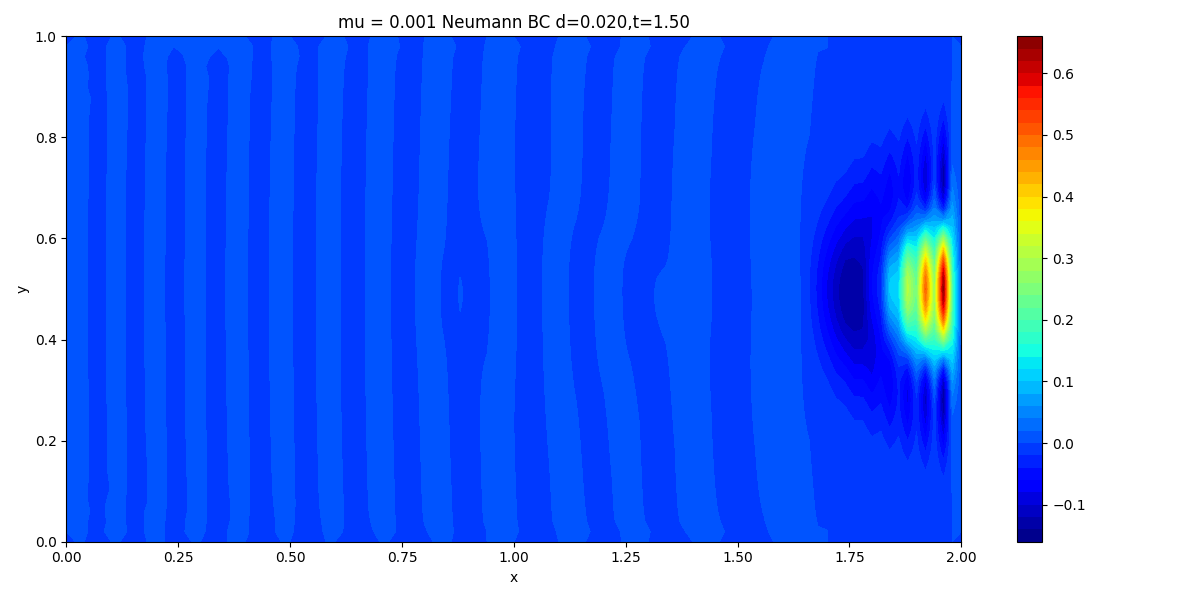
\includegraphics[width=\linewidth]{figuresmu/mu3Nud0.020t1.50.png}
    \label{fig8}
    \end{minipage}
    \vspace{-1.5em}
    
    \begin{minipage}{0.5\textwidth}
    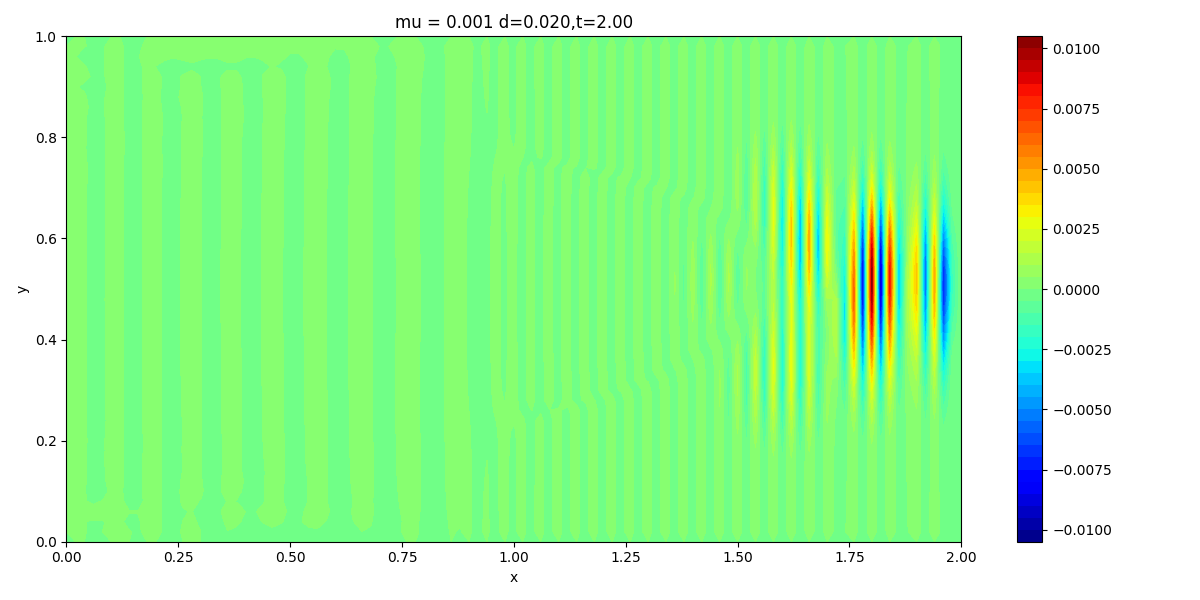
\includegraphics[width=\linewidth]{figuresmu/mu3d0.020t2.00.png}
    \label{fig9}
    \end{minipage}\hfill
    \begin{minipage}{0.5\textwidth}
    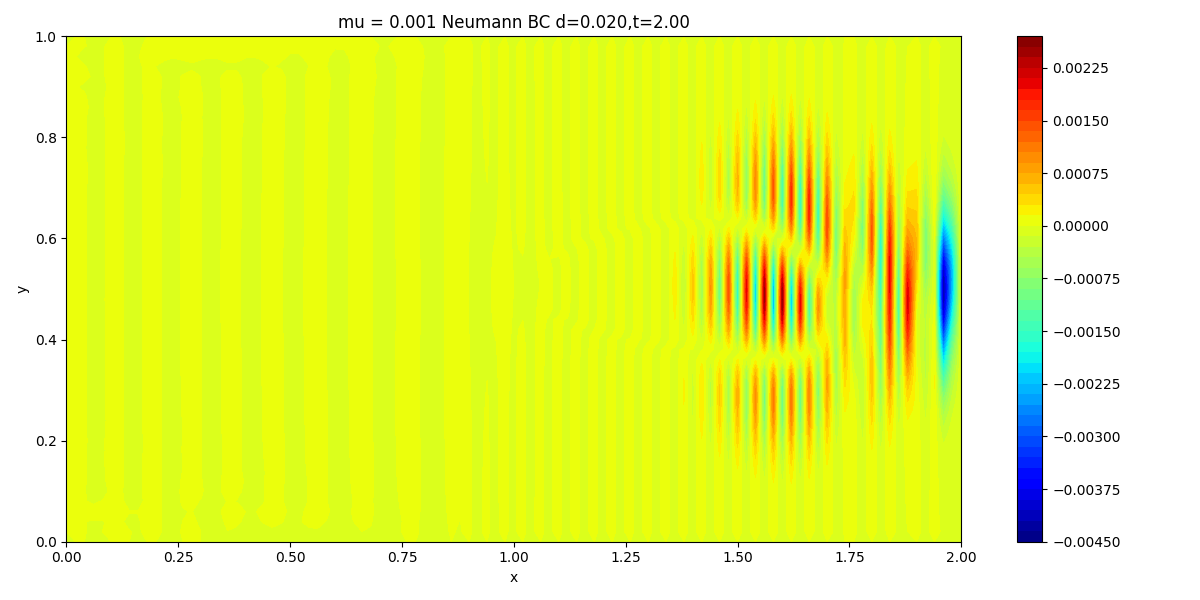
\includegraphics[width=\linewidth]{figuresmu/mu3Nud0.020t2.00.png}
    \label{fig10}
    \end{minipage}
    \caption{Grid size 0.020, $\mu = 0.001$, dirichlet BC vs Neumann BC}
    \end{minipage}
    \end{figure}


We could find the vortex is much smaller than $\mu = 0.01$ 
result, which this $\mu = 0.001$, let diffusion speed is slower.


\begin{figure}[H]
\centering
\begin{minipage}{\linewidth}
\centering
\begin{minipage}{0.5\textwidth}
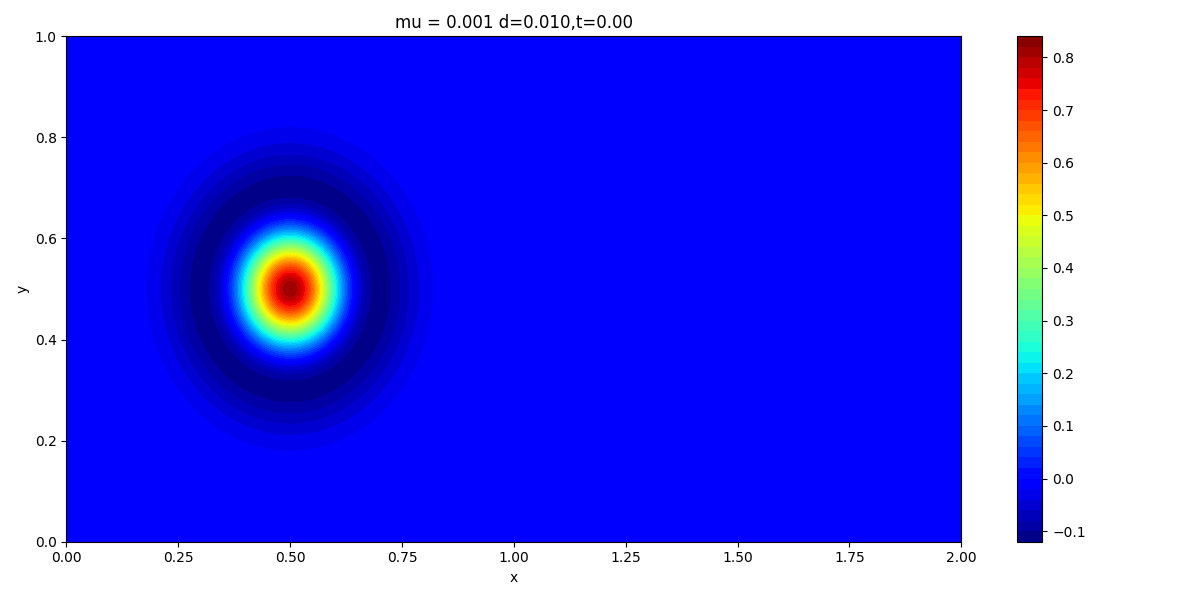
\includegraphics[width=\linewidth]{figuresmu/mu3d0.010t0.00.png}
\label{fig1}
\end{minipage}\hfill
\begin{minipage}{0.5\textwidth}
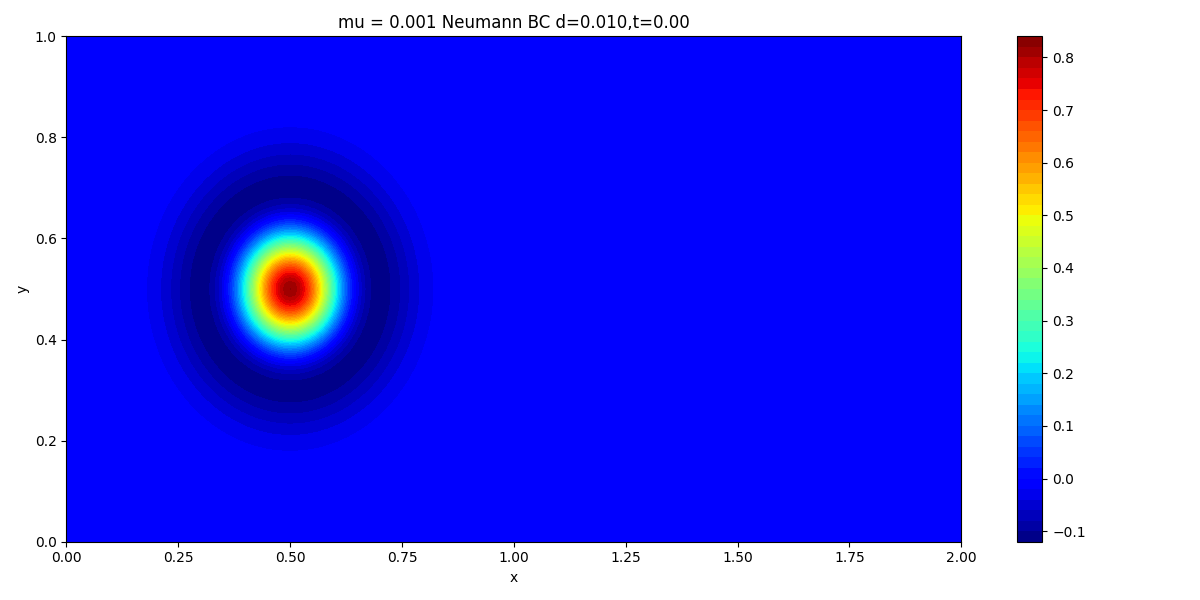
\includegraphics[width=\linewidth]{figuresmu/mu3Nud0.010t0.00.png}
\label{fig2}
\end{minipage}
\vspace{-1.5em}

\begin{minipage}{0.5\textwidth}
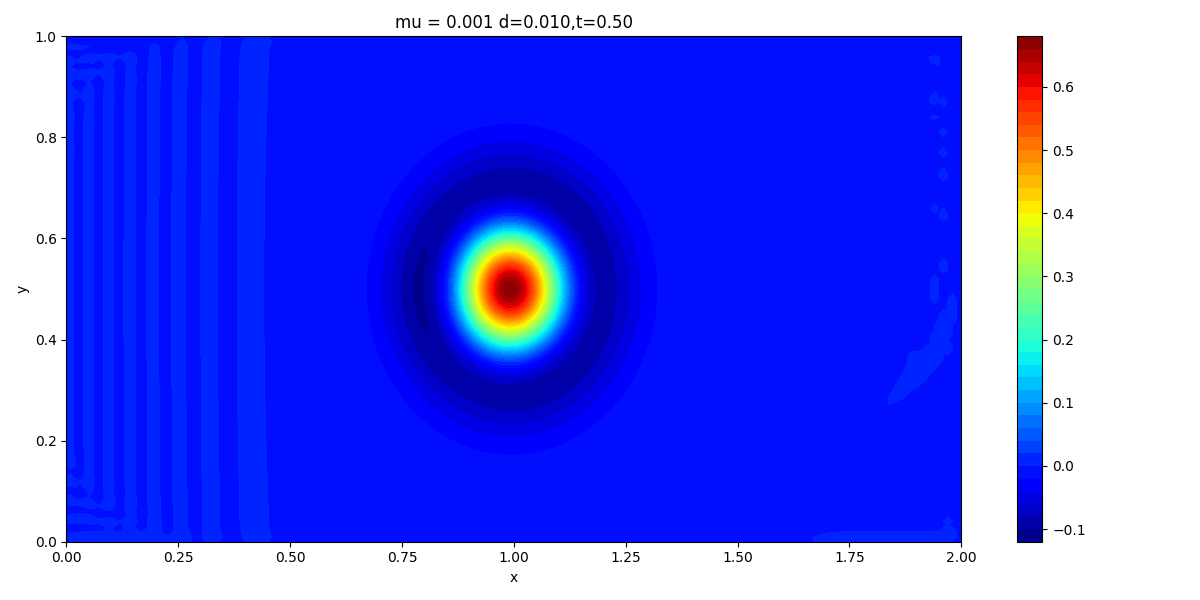
\includegraphics[width=\linewidth]{figuresmu/mu3d0.010t0.50.png}
\label{fig3}
\end{minipage}\hfill
\begin{minipage}{0.5\textwidth}
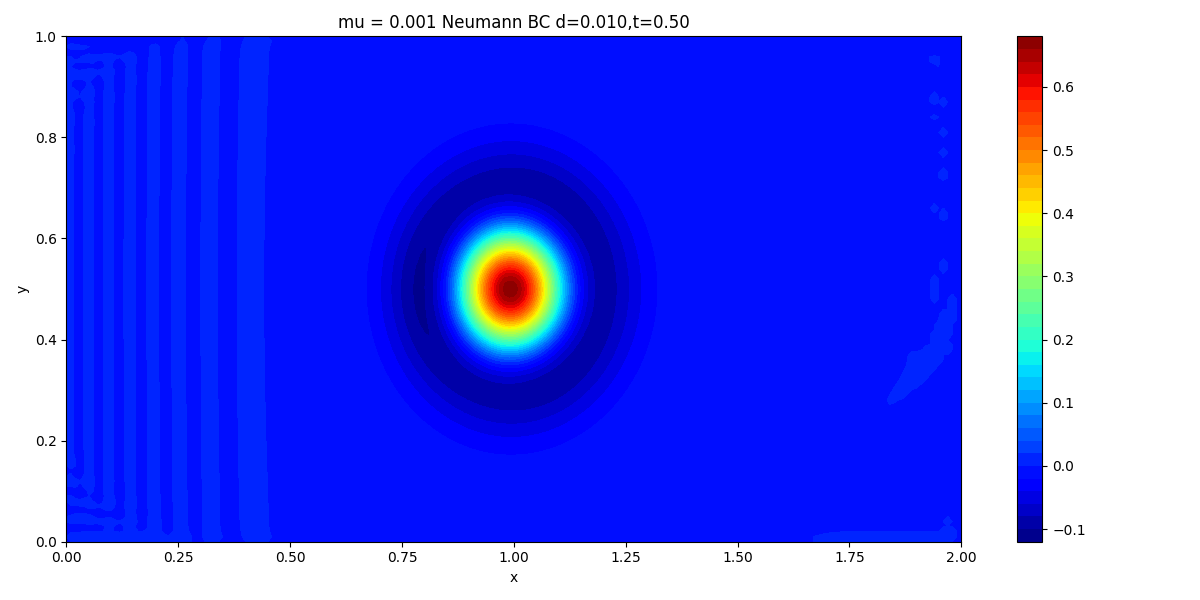
\includegraphics[width=\linewidth]{figuresmu/mu3Nud0.010t0.50.png}
\label{fig4}
\end{minipage}
\vspace{-1.5em}

\begin{minipage}{0.5\textwidth}
    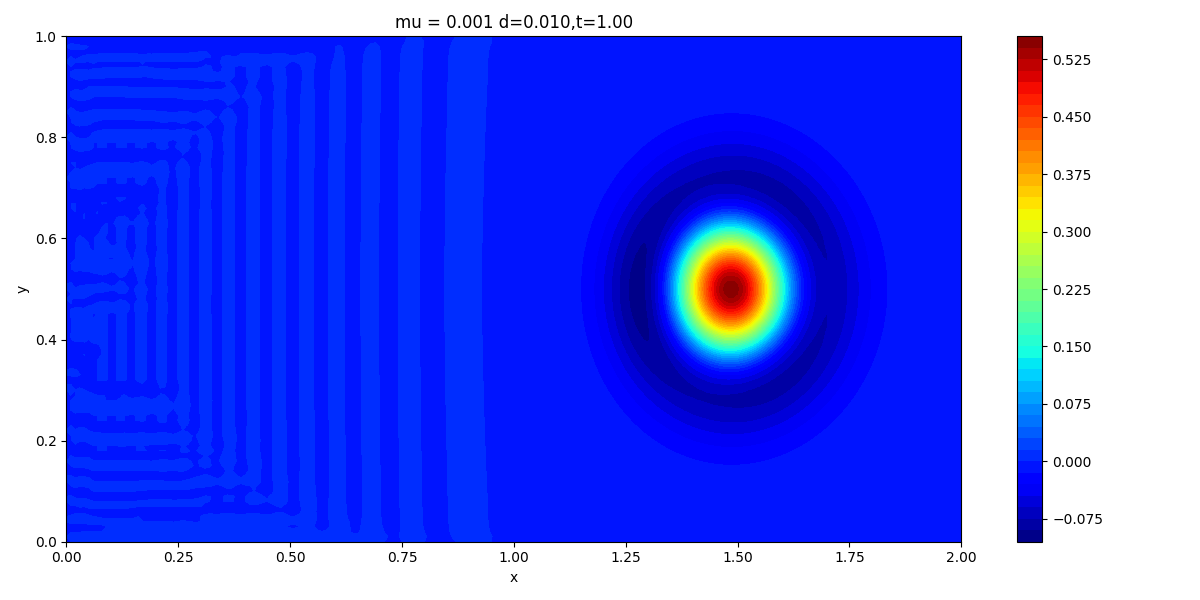
\includegraphics[width=\linewidth]{figuresmu/mu3d0.010t1.00.png}
    \label{fig3}
    \end{minipage}\hfill
    \begin{minipage}{0.5\textwidth}
    \includegraphics[width=\linewidth]{figuresmu/mu3Nud0.010t1.00.png}
    \label{fig4}
\end{minipage}
\vspace{-1.5em}

\begin{minipage}{0.5\textwidth}
\includegraphics[width=\linewidth]{figuresmu/mu3d0.010t1.50.png}
\label{fig5}
\end{minipage}\hfill
\begin{minipage}{0.5\textwidth}
\includegraphics[width=\linewidth]{figuresmu/mu3Nud0.010t1.50.png}
\label{fig6}
\end{minipage}
\vspace{-1.5em}

\begin{minipage}{0.5\textwidth}
\includegraphics[width=\linewidth]{figuresmu/mu3d0.010t2.00.png}
\label{fig7}
\end{minipage}\hfill
\begin{minipage}{0.5\textwidth}
\includegraphics[width=\linewidth]{figuresmu/mu3Nud0.010t2.00.png}
\label{fig8}
\end{minipage}
\caption{Grid size 0.010, $\mu = 0.001$, dirichlet BC vs Neumann BC}

\end{minipage}
\end{figure}






\begin{figure}[H]
    \centering
    \begin{minipage}{\linewidth}
    \centering
    \begin{minipage}{0.5\textwidth}
    \includegraphics[width=\linewidth]{figuresmu/mu3d0.005t0.00.png}
    \label{fig1}
    \end{minipage}\hfill
    \begin{minipage}{0.5\textwidth}
    \includegraphics[width=\linewidth]{figuresmu/mu3Nud0.005t0.00.png}
    \label{fig2}
    \end{minipage}
    \vspace{-1.5em}
    
    \begin{minipage}{0.5\textwidth}
    \includegraphics[width=\linewidth]{figuresmu/mu3d0.005t0.50.png}
    \label{fig3}
    \end{minipage}\hfill
    \begin{minipage}{0.5\textwidth}
    \includegraphics[width=\linewidth]{figuresmu/mu3Nud0.005t0.50.png}
    \label{fig4}
    \end{minipage}
    \vspace{-1.5em}
    
    \begin{minipage}{0.5\textwidth}
    \includegraphics[width=\linewidth]{figuresmu/mu3d0.005t1.00.png}
    \label{fig5}
    \end{minipage}\hfill
    \begin{minipage}{0.5\textwidth}
    \includegraphics[width=\linewidth]{figuresmu/mu3Nud0.005t1.00.png}
    \label{fig6}
    \end{minipage}
    \vspace{-1.5em}
    
    \begin{minipage}{0.5\textwidth}
    \includegraphics[width=\linewidth]{figuresmu/mu3d0.005t1.50.png}
    \label{fig7}
    \end{minipage}\hfill
    \begin{minipage}{0.5\textwidth}
    \includegraphics[width=\linewidth]{figuresmu/mu3Nud0.005t1.50.png}
    \label{fig8}
    \end{minipage}
    \vspace{-1.5em}
    
    \begin{minipage}{0.5\textwidth}
    \includegraphics[width=\linewidth]{figuresmu/mu3d0.005t2.00.png}
    \label{fig9}
    \end{minipage}\hfill
    \begin{minipage}{0.5\textwidth}
    \includegraphics[width=\linewidth]{figuresmu/mu3Nud0.005t2.00.png}
    \label{fig10}
    \end{minipage}
    \caption{Grid size 0.005, $\mu = 0.001$, dirichlet BC vs Neumann BC}
    \end{minipage}
    \end{figure}



\subsection{Viscus effect observation}
Compare our result in $\mu = 0.001$ and $\mu = 0.01$ (Pervious
section), we could easily observed the vortex at $\mu=0.001$
is diffused much slower than the pervious section result. In 
more detailed, is with time going, the vortex's effect range
is gowing slower, and the vortex center (peak) value remains
 larger than the $\mu = 0.01$ case. 

 \subsection{Oscillation Observation and Analysis}

 As we observed oscillation wave in the result of $\mu =0.001$,
 we also observed the oscillation effect shows more obvious
 on the coarse grid, it do not show obviously at the grid 
 size = 0.005.\\

 As we have done in HW2, we use $Pe_{\Delta x }$ to analysis
 why this effect could happen:\\

 \begin{table}[h!]
    \centering
    \renewcommand{\arraystretch}{1.5} % Adjusts the row height, default is 1
    \begin{tabular}{c|c c}
        $Pe_{\Delta x}$ & $\mu = 0.01$ & $\mu = 0.001$ \\
        \hline
        ${\Delta x}$ = 0.02 & 2 & 20 \\
        ${\Delta x}$ = 0.01 & 1 & 10 \\
        ${\Delta x}$ = 0.005 & 0.5 & 5 \\
    \end{tabular}
    \caption{$Pe_{\Delta x}$ at $U=1$ Comparison}
\end{table}


We know as the $Pe_{\Delta x}$ is pretty large, it could
cause negative term which led to oscillation. This is not
means the scheme is unstable, but the effect is unstable.\\

Compare the formal case where $\mu = 0.01$, we could find 
in this condition, the finer grid is, the low $Pe_{\Delta x}$
be, and the $Pe_{\Delta x}$ is much smaller at $\mu = 0.01$, and
become much bigger at $\mu = 0.001$, where it cause oscillation,
 could correspond to 
our case result.


% \begin{figure}[H]
%     \centering
%     \includegraphics[width=0.8\textwidth]{figures/P2U1t0.1.png}
%     \label{IGs.jpg}
%     \caption{1st UPwind scheme result }
% \end{figure}






\section{5. Accuracy \& Wavenumber Analysis}

\subsection{Modified Wavenumber}
As modified wavenumber analysis:
$$
u = u^{ik(x+y)} 
$$

Could get
$$
\frac{\partial u}{\partial x} 
= \frac{\partial u}{\partial y} = iku 
$$
$$
\frac{\partial^2 u}{\partial x^2} 
= \frac{\partial^2 u}{\partial y^2} = -k^2u 
$$


1st Central difference:
$$
\frac{\delta_x u}{\Delta x} = u\frac{u^{ik\Delta x}-u^{-ik\Delta x}}{2\Delta x} = iu\frac{\sin k\Delta x}{\Delta x} 
$$

where,
$$
k_x' = \frac{\sin k \Delta x}{\Delta x}
$$

2nd Central difference:
$$
\frac{\delta_x^2 u}{\Delta x^2} = u\frac{u^{ik\Delta x}+u^{-ik\Delta x}-2}{\Delta x^2} = u\frac{2(\cos k\Delta x-1)}{\Delta x^2} 
$$

Could get 
$$
\quad k_{xx} '= \sqrt{\frac{2(1-\cos k\Delta x)}{\Delta x^2}}
$$



The figure compare modified wavenumber and exact wavenumber
is showing below:


\begin{figure}[H]
    \centering
    \includegraphics[width=0.6\textwidth]{figuresGeneral/Midified_Wavenumber.png}
    \label{IGs.jpg}
    \caption{1st and 2nd CD Modified Wavenumber Compare to Exact }
\end{figure}


\subsection{Result Analysis with modified wavenumber}


From the figure of modified wavenumber,
we could as find the $\Delta$ getting small as we using finer 
grid, for each k, the $k\Delta x$ is moving to the left, which comming 
to the region that the scheme's modified wavenumber is closer 
to the exact wavenumber, resulted that when we using finer grid, 
the result become more accurate. \\

As the Central difference scheme's modified wavenumber only 
contains the real part, as the real part's difference make the
dispersion error, in this case specific, it make the vortex's 
wave travel faster in the same time period. More specifically, as the grid size ($\Delta$) larger, the
more diffused effect shown in the vortex, the smaller the 
peak values in the same time period.\\

This could explain the diffusion result shown in our result:
the finer the grid become, the diffusion speed comes more 
slower, matain the accuracy of the diffusion result. 

















\section{6. Effect of Outflow Boundary--Extended Boundary}

To examine the effect of the outflow condition, we use extended
domain: $x_{max}$ =3.\\


% \begin{figure}[H]
%     \includegraphics[width=0.6\linewidth]{figures/3d0.02t1.50.png}\\
%     \label{IGs.jpg}
% \end{figure}

% \vspace{-3.5em}


% \begin{figure}[H]
%     \includegraphics[width=0.6\linewidth]{figures/3Ed0.020t1.50.png}\\
%     \label{IGs.jpg}
% \end{figure}

% \vspace{-3.5em}


% \begin{figure}[H]
%     \includegraphics[width=0.9\linewidth]{figures6/3Ed0.020t1.50Ext.png}
%     \label{IGs.jpg}
%     \caption{Comparsion of Dirichlet BC reuslt, Neumann BC result, and Extended outflow result}
% \end{figure}





% The comparsion at t=1.5, d=0.02 is showing below:
% \begin{figure}[H]
%     \includegraphics[width=0.6\linewidth]{figures/3d0.02t1.50.png}\\
%     \includegraphics[width=0.6\linewidth]{figures/3Ed0.020t1.50.png}\\
%     \includegraphics[width=0.9\linewidth]{figures6/3Ed0.020t1.50Ext.png}
%     \label{IGs.jpg}
%     \caption{Comparsion of Dirichlet BC reuslt, Neumann BC result, and Extended outflow result}
% \end{figure}



The comparsion at t=1.5, d=0.02 is showing below:
\begin{figure}[H]
    \includegraphics[width=0.6\linewidth]{figures/3d0.01t1.50.png}\\
    \includegraphics[width=0.6\linewidth]{figures/3Ed0.010t1.50.png}\\
    \includegraphics[width=0.9\linewidth]{figures6/6d0.010t1.50.png}
    \label{IGs.jpg}
    \caption{Comparsion of Dirichlet BC reuslt, Neumann BC result, and Extended outflow result}
\end{figure}

We could find that the extended domain result is much similiar
to the Neumann Boundary condition, where the vortex do not been
enormouslly impacted by the artifically boundary.\\

For more specific analysis, the Dirichlet boundary condition 
artifically set the outflow condition on the boundary is not
effected by the flow condition inside, which in this case is 
our vortex. In Neumann boundary condition, it sets the boundary
is effected by the flow condition inside the domain, which could
more fit the vortex propagation without artifically boundary effect.



\begin{figure}[H]
    \includegraphics[width=1.8\linewidth]{figures6/6dE20.010t1.5.png}
    \label{IGs.jpg}
    \caption{Extended outflow to x=6 result}
\end{figure}

We also examined much more larger domain ($x_max = 6$), could 
also show is much similiar to the Neumann boundary condition,
where the boundary do not have much artifically effect to the 
flow condition inside, where makes it could simulate kind
of free-flow condition


% \begin{figure}[H]
%     \includegraphics[width=0.6\linewidth]{figures/3d0.01t2.00.png}\\
%     \includegraphics[width=0.6\linewidth]{figures/3Ed0.010t2.00.png}\\
%     \includegraphics[width=0.9\linewidth]{figures6/6dE10.010t2.0.png}
%     \label{IGs.jpg}
%     \caption{Comparsion of Dirichlet BC reuslt, Neumann BC result, and Extended outflow result}
% \end{figure}
\section{Conclusion}


In this project, we discretized the viscous Burgers' equation 
using the Central Difference scheme for 
spatial differentiation, the Forward Euler for 
the convection term, and the Backward Euler for 
the diffusion term to handle temporal derivatives. 
We then employed ADI solver 
to obtain a tridiagonal matrix, which updat3 by 
lines at first half
time step and update by columns at the second time step.
 We then implemented 
 TDMA to solve the tridiagonal matrix and derive the results.\\

We investigated the effects of grid size, boundary conditions,
 and viscosity on the outcomes, also the effect of the 
 $Pe_{\Delta x}$. Our findings indicate that as 
 the grid becomes finer, diffusion tends to be slower 
 and less pronounced, mirroring the impact of reduced viscosity.
However, $Pe_{\Delta x}$ too large could also cause oscillation,
where shown in the result of $\mu = 0.001$, the large the grid size we set, the 
smaller $\mu$ we use, the large $Pe_{\Delta x}$
we get, and the large oscillation we obtained.\\


We also compared the effects of Dirichlet and 
Neumann boundary conditionswhere Neumann boundary condition 
shows more close
to the accurate result as the interior flow do not hugely 
effected by the artifically limit of the domain like Dirichlet 
boundary condition.



%%%%%%%%%%%%%%%%%%%%%%%%%%%%%%%%%%%%%%%%%%%%%%%%%%%%%%%%%%%%%%%















% \begin{figure}[H]
%     \centering
%     \includegraphics[width=0.8\textwidth]{figures/P2U1t0.1.png}
%     \label{IGs.jpg}
%     \caption{1st UPwind scheme result }
% \end{figure}





%%%%%%%%%%%%%%%%%%%%%%%%%%%%%%%%%%%%%%%%%%%%%%%%%%%%%%%%%%%%%%%
%%%%%%%%%%%%%%%%%%%%%%%%%%%%%%%%%%%%%%%%%%%%%%%%%%%%%%%%%%%%%%%
%%%%%%%%%%%%%%%%%%%%%%%%%%%%%%%%%%%%%%%%%%%%%%%%%%%%%%%%%%%%%%%
\newpage
\section*{Appendix}
% 在目录中添加Appendix
\addcontentsline{toc}{section}{Appendix}
\begin{scriptsize}

\begin{lstlisting}[language=python,caption={ADI Solver}]

    import numpy as np #use it in all class u,v

    import math # use it in Init to get initial value
    import copy # use it in TDMA and Update to avoid influence origional data
    
    import matplotlib.pyplot as plt  # use it to draw vorticity contour
    
    
    
    def TDMA(a, b, c, d):  
              # TDMA solver 
              # b: main diagional  a: down diaginoal c: up diagional 
              # lenth of a , b, c, d is as same as D, with no use of a[0], a[max], c[0], c[max]
               
                    # | b0  c0   0  ...   0   |
                    # | a1  b1  c1  ...   0   |
                    # |  0  a2  b2  ...   0   |
                    # | ... ... ... ...  ...  |
                    # |  0  ... an-2 bn-2 cn-2|
                    # |  0  ...  0   an-1 bn-1|
    
        import copy
        do = copy.deepcopy(d)
        ao = copy.deepcopy(a)
        bo = copy.deepcopy(b)
        co = copy.deepcopy(c)
        N = len(d)
        xo = np.zeros(N)
        
        for rowi in range(1,N):
            k = ao[rowi]/bo[rowi-1]
            bo[rowi] -= co[rowi-1]*k
            do[rowi] -= do[rowi-1]*k
        
        xo[N-1] = do[N-1]/bo[N-1]
        for rowi in range(N-2,-1,-1):
            xo[rowi] = (do[rowi]-co[rowi]*xo[rowi+1])/bo[rowi]
    
        return xo
    
    
    
    class ADI_Solver:
        def __init__(self, x_max, y_max, t_max, dx, dy, dt, mu):
            self.x_max = x_max
            self.y_max = y_max
            self.t_max = t_max
            self.dx = dx
            self.dy = dy
            self.dt = dt
            self.mu = mu
    
        def  Grid_Generate(self):
            self.i_max = int(self.x_max/self.dx)
            self.j_max = int(self.y_max/self.dy)
            self.n_max = int(self.t_max/self.dt)
    
            self.u = np.zeros([ self.i_max+1 , self.j_max+1 ], dtype = float)
            self.v = np.zeros([ self.i_max+1 , self.j_max+1 ], dtype = float)
    
    
        def Initialize(self):
            for i in range(0, self.i_max+1):
                for j in range(0, self.j_max+1):
                    self.u[i][j], self.v[i][j] = self.initial_formula(i, j)
    
            # print(self.u) ## TESTING 
    
        def initial_formula(self, i, j):
            V_t = 0.25
            x_0 = 0.5
            y_0 = 0.5
            r_0 = 0.1
    
            r2 = (i*self.dx-x_0)**2+(j*self.dy-y_0)**2
    
            u_init = 1 - V_t * (j*self.dy-y_0) * math.exp( (1-( r2 )/(r_0**2)) / (2) )
            v_init = V_t * (i*self.dx-x_0) * math.exp( (1-( r2 )/(r_0**2)) / (2) )
    
            return u_init, v_init
        
    
        def BC(self, u , v):
    
            for i in range(0, self.i_max+1):
                u[i][0] = 1
                v[i][0] = 0
                u[i][-1] = 1
                v[i][-1] = 0
            
            for j in range(0, self.j_max+1):
                u[0][j] = 1
                v[0][j] = 0
                u[-1][j] = 1
                v[-1][j] = 0
                # u[self.i_max-1][j], v[self.i_max-1][j] = u[self.i_max][j], v[self.i_max][j]
            return u, v
        
    
        def Iterative(self):
            self.u, self.v = self.BC(self.u, self.v)
            
            for n in range(0,self.n_max):
                self.u, self.v = self.BC(self.u, self.v)
                
                u_new, v_new = copy.deepcopy(self.u), copy.deepcopy(self.v)
                
                u_new, v_new = self.K_iteration(self.u, self.v)
    
                self.u, self.v = u_new, v_new
                print(n)
            
            return self.u, self.v
                     
    
    
    
    
    
    
        def K_iteration(self, u, v):
    
            u_half, v_half = copy.deepcopy(u), copy.deepcopy(v)
            u_new, v_new =  copy.deepcopy(u), copy.deepcopy(v)
    
    
                # update u:
                    # u{n} to u{n+1/2} line update:
            for j in range(1, self.j_max):  # flag=flag(0/1,0/1), 1:donig 0:other
                flag = (0,1)
                u_half[:,j] = self.UPdate( u , v, u, j, self.i_max, flag)
                    # Update function: Update(u, v, doing(u/v), doing(row=j/column=i), doingAnother, flag)
                
    
    
            u_new, v_new = self.BC(u_new, v_new)
            u_half, v_half = self.BC(u_half, v_half )
                
            
                # update v:
            for j in range(1, self.j_max):  # flag=flag(0/1,0/1), 1:donig 0:other
                flag = (0,1)
                v_half[:,j] = self.UPdate( u_half , v, v, j, self.i_max, flag)
            
    
            u_new, v_new = self.BC(u_new, v_new)
            u_half, v_half = self.BC(u_half, v_half )
    
                    
                    # u{n+1/2} to u{n+1} column update:
            for i in range(1,self.i_max-1):
                flag = (1,0)
                u_new[i,:] = self.UPdate( u_half , v_half, u_half, i, self.j_max, flag)
            
    
            u_new, v_new = self.BC(u_new, v_new)
            u_half, v_half = self.BC(u_half, v_half )
                
    
    
            for i in range(1,self.i_max):
                flag = (1,0)
                v_new[i,:] = self.UPdate( u_new , v_half , v_half, i, self.j_max, flag)
            
    
            u_new, v_new = self.BC(u_new, v_new)
            u_half, v_half = self.BC(u_half, v_half )
    
            return u_new , v_new
        
    
        def UPdate(self, u, v, U,  Idoing, Ianother_max, flag):
    
            delta = self.dx * flag[1] + self.dy*flag[0]
    
    
            r = (self.mu*self.dt)/(2*delta**2)
    
    
            # Creating a, b, c, D
            a = np.full(Ianother_max-1, -r, dtype = float)
            b = np.full(Ianother_max-1, 1 + 4*r, dtype = float)
            c = np.full(Ianother_max-1, -r, dtype = float)
            d = np.full(Ianother_max+1, 0, dtype = float)
    
            for ij in range(1,Ianother_max):
                i,j = Idoing*flag[0] + ij* flag[1] ,Idoing*flag[1] + ij* flag[0]
                cox = (u[i,j]*self.dt/self.dx /2)
                coy = (v[i,j]*self.dt/self.dy /2)
                rx = (self.mu*self.dt/(2*self.dx**2))
                ry = (self.mu*self.dt/(2*self.dy**2))
                rxy = rx * flag[1] + ry*flag[0]
                d[ij] = U[i,j]-cox*((U[i+1,j]-U[i-1,j])/(2))-coy*((U[i,j+1]-U[i,j-1])/(2))+rxy*(U[i+flag[0],j+flag[1]]+U[i-flag[0],j-flag[1]])
            d[0], d[-1] = U[i*flag[0],j*flag[1]], U[i*flag[0]-1,j*flag[1]-1]
            
            
            # added boundary get full matrix:
            a = np.concatenate((np.array([0]), a, np.array([0])), axis=0)
            b = np.concatenate((np.array([1]), b, np.array([1])), axis=0)
            c = np.concatenate((np.array([0]), c, np.array([0])), axis=0)
    
    
               
            u_UPdate = TDMA(a, b, c, d)
    
                # | 1   0    0   ...   0      0    |
                # | a1  b1  c1   ...   0      0    |
                # |  0  a2  b2   ...   0      0    |
                # | ... ... ...  ...  ...    ...   |
                # |  0  0    0   ...  b(n-2) c(n-2)|
                # |  0  0    0   ...   0      1    |
            
            # print("TDMA")
            # print(u_UPdate)
    
            return u_UPdate
    
    
    
    
    
    
    def Do_Solver(x_max, y_max, t_max, dx, dy, dt , mu):
         
        Try_1  = ADI_Solver(x_max, y_max, t_max, dx, dy, dt , mu)
        Try_1.Grid_Generate()
        Try_1.Initialize()
        u, v =Try_1.Iterative()
    
        return u,v
    
    
    def Vorticity(u, v, t):
        # u,v = np.transpose(u), np.transpose(v)
    
        Ni, Nj = u.shape
    
        x = np.linspace(0, 2, Ni)
        y = np.linspace(0, 1, Nj)
    
        X, Y = np.meshgrid(x, y)
    
        omega = np.zeros((Ni, Nj))
        # omega[1:-1, 1:-1] = (v[1:-1, 2:] - v[1:-1, :-2]) / (x[2] - x[1]) - (u[2:, 1:-1] - u[:-2, 1:-1]) / (y[2] - y[1])
    
        for i in range(1,Ni-1):
             for j in range(1,Nj-1):
                  omega[i,j] = (v[i+1,j] - v[i-1,j])/(x[2]-x[0])-(u[i,j+1] - u[i,j-1])/(y[2] - y[0])
        
        omega = np.transpose(omega)
    
    
    
        d = x[2]-x[1]
    
        print(d)
    
        plt.figure(figsize=(12, 6))
        plt.contourf(X, Y, omega, levels=50, cmap='jet')
        plt.colorbar()
        plt.title('d={:.3f},t={:.2f}'.format(d,t))
        plt.xlabel('x')
        plt.ylabel('y')
    
    
        plt.tight_layout()
        plt.savefig('3d{:.3f}t{:.2f}.png'.format(d,t))
        # plt.show()
    
        
    
    
    def main():
        x_max =2
        y_max =1
        t_max = 2
    
        # dx = 0.02
        # dy = 0.01
        # dt = 0.005
    
    
        dx = 0.005
        dy = 0.005
        dt = 0.001
    
    
        mu = 0.01
        # mu = 1
    
    
        t_max = 0
        u,v = Do_Solver(x_max, y_max, t_max, dx, dy, dt , mu)
        # print(u)
        Vorticity(u, v, t_max)
    
        t_max = 0.5
        u,v = Do_Solver(x_max, y_max, t_max, dx, dy, dt , mu)
        # print(u)
        Vorticity(u, v, t_max)
    
        t_max = 1
        u,v = Do_Solver(x_max, y_max, t_max, dx, dy, dt , mu)
        # print(u)
        Vorticity(u, v, t_max)
    
        t_max = 1.5
        u,v = Do_Solver(x_max, y_max, t_max, dx, dy, dt , mu)
        # print(u)
        Vorticity(u, v, t_max)
    
        t_max = 2
        u,v = Do_Solver(x_max, y_max, t_max, dx, dy, dt , mu)
        # print(u)
        Vorticity(u, v, t_max)
    
    
    
    if __name__ == '__main__':
         main()
        # arg1 = [2,2,2,2,2]
        # arg2 = [1,1,1,1,1]
        # arg3 = arg1
        # arg4 = [1,2,3,4,5]
        # print(TDMA(arg1,arg2,arg3,arg4))
    

\end{lstlisting}




\begin{lstlisting}[language=python,caption={Extended Region using ADI Solver}]


    import numpy as np #use it in all class u,v

    import math # use it in Init to get initial value
    import copy # use it in TDMA and Update to avoid influence origional data
    
    import matplotlib.pyplot as plt  # use it to draw vorticity contour
    
    
    
    def TDMA(a, b, c, d):  
              # TDMA solver 
              # b: main diagional  a: down diaginoal c: up diagional 
              # lenth of a , b, c, d is as same as D, with no use of a[0], a[max], c[0], c[max]
               
                    # | b0  c0   0  ...   0   |
                    # | a1  b1  c1  ...   0   |
                    # |  0  a2  b2  ...   0   |
                    # | ... ... ... ...  ...  |
                    # |  0  ... an-2 bn-2 cn-2|
                    # |  0  ...  0   an-1 bn-1|
    
        import copy
        do = copy.deepcopy(d)
        ao = copy.deepcopy(a)
        bo = copy.deepcopy(b)
        co = copy.deepcopy(c)
        N = len(d)
        xo = np.zeros(N)
        
        for rowi in range(1,N):
            k = ao[rowi]/bo[rowi-1]
            bo[rowi] -= co[rowi-1]*k
            do[rowi] -= do[rowi-1]*k
        
        xo[N-1] = do[N-1]/bo[N-1]
        for rowi in range(N-2,-1,-1):
            xo[rowi] = (do[rowi]-co[rowi]*xo[rowi+1])/bo[rowi]
    
        return xo
    
    
    
    class ADI_Solver:
        def __init__(self, x_max, y_max, t_max, dx, dy, dt, mu):
            self.x_max = x_max
            self.y_max = y_max
            self.t_max = t_max
            self.dx = dx
            self.dy = dy
            self.dt = dt
            self.mu = mu
    
        def  Grid_Generate(self):
            self.i_max = int(self.x_max/self.dx)
            self.j_max = int(self.y_max/self.dy)
            self.n_max = int(self.t_max/self.dt)
    
            self.u = np.zeros([ self.i_max+1 , self.j_max+1 ], dtype = float)
            self.v = np.zeros([ self.i_max+1 , self.j_max+1 ], dtype = float)
    
    
        def Initialize(self):
            for i in range(0, self.i_max+1):
                for j in range(0, self.j_max+1):
                    self.u[i][j], self.v[i][j] = self.initial_formula(i, j)
    
            # print(self.u) ## TESTING 
    
        def initial_formula(self, i, j):
            V_t = 0.25
            x_0 = 0.5
            y_0 = 0.5
            r_0 = 0.1
    
            r2 = (i*self.dx-x_0)**2+(j*self.dy-y_0)**2
    
            u_init = 1 - V_t * (j*self.dy-y_0) * math.exp( (1-( r2 )/(r_0**2)) / (2) )
            v_init = V_t * (i*self.dx-x_0) * math.exp( (1-( r2 )/(r_0**2)) / (2) )
    
            return u_init, v_init
        
    
        def BC(self, u , v):
    
            for i in range(0, self.i_max+1):
                u[i][0] = 1
                v[i][0] = 0
                u[i][-1] = 1
                v[i][-1] = 0
            
            for j in range(0, self.j_max+1):
                u[0][j] = 1
                v[0][j] = 0
                u[-1][j] = 1
                v[-1][j] = 0
                # u[self.i_max-1][j], v[self.i_max-1][j] = u[self.i_max][j], v[self.i_max][j]
            return u, v
        
    
        def Iterative(self):
            self.u, self.v = self.BC(self.u, self.v)
            
            for n in range(0,self.n_max):
                self.u, self.v = self.BC(self.u, self.v)
                
                u_new, v_new = copy.deepcopy(self.u), copy.deepcopy(self.v)
                
                u_new, v_new = self.K_iteration(self.u, self.v)
    
                self.u, self.v = u_new, v_new
                print(n)
            
            return self.u, self.v
                     
    
    
    
    
    
    
        def K_iteration(self, u, v):
    
            u_half, v_half = copy.deepcopy(u), copy.deepcopy(v)
            u_new, v_new =  copy.deepcopy(u), copy.deepcopy(v)
    
    
                # update u:
                    # u{n} to u{n+1/2} line update:
            for j in range(1, self.j_max):  # flag=flag(0/1,0/1), 1:donig 0:other
                flag = (0,1)
                u_half[:,j] = self.UPdate( u , v, u, j, self.i_max, flag)
                    # Update function: Update(u, v, doing(u/v), doing(row=j/column=i), doingAnother, flag)
                
    
    
            u_new, v_new = self.BC(u_new, v_new)
            u_half, v_half = self.BC(u_half, v_half )
                
            
                # update v:
            for j in range(1, self.j_max):  # flag=flag(0/1,0/1), 1:donig 0:other
                flag = (0,1)
                v_half[:,j] = self.UPdate( u_half , v, v, j, self.i_max, flag)
            
    
            u_new, v_new = self.BC(u_new, v_new)
            u_half, v_half = self.BC(u_half, v_half )
    
                    
                    # u{n+1/2} to u{n+1} column update:
            for i in range(1,self.i_max-1):
                flag = (1,0)
                u_new[i,:] = self.UPdate( u_half , v_half, u_half, i, self.j_max, flag)
            
    
            u_new, v_new = self.BC(u_new, v_new)
            u_half, v_half = self.BC(u_half, v_half )
                
    
    
            for i in range(1,self.i_max):
                flag = (1,0)
                v_new[i,:] = self.UPdate( u_new , v_half , v_half, i, self.j_max, flag)
            
    
            u_new, v_new = self.BC(u_new, v_new)
            u_half, v_half = self.BC(u_half, v_half )
    
            return u_new , v_new
       
    
        def UPdate(self, u, v, U,  Idoing, Ianother_max, flag):
    
            delta = self.dx * flag[1] + self.dy*flag[0]
    
    
            r = (self.mu*self.dt)/(2*delta**2)
    
    
            # Creating a, b, c, D
            a = np.full(Ianother_max-1, -r, dtype = float)
            b = np.full(Ianother_max-1, 1 + 4*r, dtype = float)
            c = np.full(Ianother_max-1, -r, dtype = float)
            d = np.full(Ianother_max+1, 0, dtype = float)
    
            for ij in range(1,Ianother_max):
                i,j = Idoing*flag[0] + ij* flag[1] ,Idoing*flag[1] + ij* flag[0]
                cox = (u[i,j]*self.dt/self.dx /2)
                coy = (v[i,j]*self.dt/self.dy /2)
                rx = (self.mu*self.dt/(2*self.dx**2))
                ry = (self.mu*self.dt/(2*self.dy**2))
                rxy = rx * flag[1] + ry*flag[0]
                d[ij] = U[i,j]-cox*((U[i+1,j]-U[i-1,j])/(2))-coy*((U[i,j+1]-U[i,j-1])/(2))+rxy*(U[i+flag[0],j+flag[1]]+U[i-flag[0],j-flag[1]])
            d[0], d[-1] = U[i*flag[0],j*flag[1]], U[i*flag[0]-1,j*flag[1]-1]
            
            
            # added boundary get full matrix:
            a = np.concatenate((np.array([0]), a, np.array([0])), axis=0)
            b = np.concatenate((np.array([1]), b, np.array([1])), axis=0)
            c = np.concatenate((np.array([0]), c, np.array([0])), axis=0)
    
    
               
            u_UPdate = TDMA(a, b, c, d)
    
                # | 1   0    0   ...   0      0    |
                # | a1  b1  c1   ...   0      0    |
                # |  0  a2  b2   ...   0      0    |
                # | ... ... ...  ...  ...    ...   |
                # |  0  0    0   ...  b(n-2) c(n-2)|
                # |  0  0    0   ...   0      1    |
            
            # print("TDMA")
            # print(u_UPdate)
    
            return u_UPdate
    
    
    
    
    
    
    def Do_Solver(x_max, y_max, t_max, dx, dy, dt , mu):
         
        Try_1  = ADI_Solver(x_max, y_max, t_max, dx, dy, dt , mu)
        Try_1.Grid_Generate()
        Try_1.Initialize()
        u, v =Try_1.Iterative()
    
        return u,v
    
    
    def Vorticity(u, v, t):
        # u,v = np.transpose(u), np.transpose(v)
    
        Ni, Nj = u.shape
    
        x = np.linspace(0, 3, Ni)
        y = np.linspace(0, 1, Nj)
    
        X, Y = np.meshgrid(x, y)
    
        omega = np.zeros((Ni, Nj))
        # omega[1:-1, 1:-1] = (v[1:-1, 2:] - v[1:-1, :-2]) / (x[2] - x[1]) - (u[2:, 1:-1] - u[:-2, 1:-1]) / (y[2] - y[1])
    
        for i in range(1,Ni-1):
             for j in range(1,Nj-1):
                  omega[i,j] = (v[i+1,j] - v[i-1,j])/(x[2]-x[0])-(u[i,j+1] - u[i,j-1])/(y[2] - y[0])
        
        omega = np.transpose(omega)
    
    
    
        d = x[2]-x[1]
    
        print(d)
    
        plt.figure(figsize=(18, 6))
        plt.contourf(X, Y, omega, levels=50, cmap='jet')
        plt.colorbar()
        plt.title('d={:.3f},t={:.2f}'.format(d,t))
        plt.xlabel('x')
        plt.ylabel('y')
    
    
        plt.tight_layout()
        plt.savefig('6d{:.3f}t{:.2f}.png'.format(d,t))
        plt.show()
    
        
    
    
    def main():
        x_max =3
        y_max =1
        t_max = 1.5
    
        # dx = 0.02
        # dy = 0.01
        # dt = 0.005
    
    
        dx = 0.01
        dy = 0.01
        dt = 0.001
    
    
        mu = 0.01
        # mu = 1
    
    
        u,v = Do_Solver(x_max, y_max, t_max, dx, dy, dt , mu)
        # print(u)
        Vorticity(u, v, t_max)
    
    
    
    if __name__ == '__main__':
         main()
        # arg1 = [2,2,2,2,2]
        # arg2 = [1,1,1,1,1]
        # arg3 = arg1
        # arg4 = [1,2,3,4,5]
        # print(TDMA(arg1,arg2,arg3,arg4))
    
    
    
    
    
    


\end{lstlisting}

















\end{scriptsize}




%%%%%%%%%%%%%%%%%%%%%%%%%%%%%%%%%%%%%%%%%%%%%%%%%%%%%%%%%%%%%%%
%%%%%%%%%%%%%%%%%%%%%%%%%%%%%%%%%%%%%%%%%%%%%%%%%%%%%%%%%%%%%%%
%%%%%%%%%%%%%%%%%%%%%%%%%%%%%%%%%%%%%%%%%%%%%%%%%%%%%%%%%%%%%%%



\end{document}